%  LaTeX support: latex@mdpi.com 
%  For support, please attach all files needed for compiling as well as the log file, and specify your operating system, LaTeX version, and LaTeX editor.

%=================================================================
\documentclass[remotesensing,article,submit,moreauthors]{Definitions/mdpi} 
%\documentclass[journal,article,submit,moreauthors,unicode]{Definitions/mdpi} % For some letters Palatino lacks
%\documentclass[preprints,article,submit,moreauthors]{Definitions/mdpi} 
%\documentclass[preprints,article,submit,moreauthors,unicode]{Definitions/mdpi} 
% For posting an early version of this manuscript as a preprint, you may use "preprints" as the journal. Changing "submit" to "accept" before posting will remove line numbers.

%--------------------
% Class Options:
%--------------------
%----------
% journal
%----------
% Choose between the following MDPI journals:
% aam, aamr, aapm, acbr, accountaudit, acn, acoustics, actuators, addictions, addictprev, adhesives, adolescents, aee, aep, aerobiology, aeronautics, aerospace, agriculture, agriengineering, agrochemicals, agronomy, ai, aiaerosp, aiagents, aibiol, aichem, aieng, aimater, aimed, aipa, air, aisens, aisoc, aiua, algorithms, allergies, alloys, amh, analog, analytica, analytics, anatomia, anesthres, animals, antibiotics, antibodies, antioxidants, applbiosci, appliedchem, appliedmath, appliedphys, applmech, applmicrobiol, applnano, applsci, aps, aquacj, archaeolstud, architecture, arm, arthropoda, asc, asd, asi, astronautics, astronomy, atmosphere, atoms, audiolres, automation, axioms, bacteria, batteries, bcrc, bdcc, beverages, bioactives, biochem, bioengineering, biologics, biology, biomass, biomechanics, biomed, biomedicines, biomedinformatics, biomimetics, biomolecules, biophysica, bioresourbioprod, biosensors, biosphere, biotech, birds, blockchains, bloods, blsf, brainsci, breath, bse, buildings, cancers, carbon, cardio, cardiogenetics, cardiovascmed, catalysts, cdr, cells, ceramics, challenges, chemeco, chemengineering, chemistry, chemosensors, chemproc, children, chips, cimb, civileng, cleantechnol, climate, clinbioenerg, clinpract, clockssleep, cmd, cmtr, coasts, coatings, colloids, colorants, complexities, complications, compounds, computation, computers, condensedmatter, conservation, constrmater, cosmetics, covid, crops, cryo, cryptography, crystals, csmf, ctn, culture, curroncol, cyber, dairy, data, ddc, dentistry, dermato, dermatopathology, designs, devices, dgg, dhi, diabetology, diagnostics, dietetics, digital, disabilities, diseases, diversity, dna, drones, drugreact, drylandsci, dynamics, earth, ebj, ece, ecm, eco-environsci, ecologies, edm, eesp, electricity, electrochem, electronicmat, electronics, embodiedintell, encyclopedia, endocrines, energies, eng, engproc, entomology, entropy, environments, environremediat, enzymology, epidemiologia, epigenomes, epilepsy, esa, est, fermentation, fibers, fintech, fire, fishes, fluids, foodeng, foods, forecasting, forensicsci, forests, fossstud, foundations, fractalfract, freshwater, fuels, future, futureinternet, futurepharmacol, futurephys, futuretransp, galaxies, gases, gastroent, gastrointestdisord, gastronomy, gels, genes, geochem, geographies, geohazards, geomatics, geometry, geosciences, geotechnics, geriatrics, germs, glacies, grainsci, grasses, green, greenhealth, gucdd, gynecolcancer, hardware, hazardousmatters, healthcare, healthcmater, hearts, hemato, hematolrep, hep, heritage, higheredu, highthroughput, hls, horticulturae, hospitals, humanoids, hydrobiology, hydrogen, hydrology, hydrometeorology, hydropower, hygiene, idhm, idr, iic, ijem, ijerph, ijgi, ijmd, ijms, ijns, ijom, ijp, ijpb, ijt, ijtm, ijtpp, ijtst, ime, immuno, industries, inflammj, informatics, information, infrastructures, inorganics, insects, instruments, inventions, iot, iron, j, jaestheticmed, jal, japma, jcdd, jcm, jcp, jcrm, jcs, jcto, jdad, jdb, jdcp, jdream, jemr, jeta, jfb, jfmk, jfth, jgbg, jgg, jimaging, jissn, jlpea, jmahp, jmmp, jmms, jmp, jmse, jne, jnt, jof, joitmc, joma, jop, joptm, jor, jox, jpbi, jphytomed, jpm, jsan, jtaer, jvd, jzbg, kidneydial, kinasesphosphatases, knowledge, labmed, laboratories, lam, land, langtechnol, lasers, legumes, life, lights, limnolrev, lipidology, liquids, livers, logics, logistics, lubricants, lymphatics, machines, macromol, magnetism, magnetochemistry, make, marinedrugs, maritime, materials, materproc, mathematics, mca, mcb, measurements, meb, medicina, medicines, medsci, membranes, merits, metabolites, metals, metamaterialsadv, meteorology, methane, metrics, metrology, micro, microarrays, microbiolres, microchem, microelectronics, micromachines, microorganisms, microplastics, microwave, minerals, mining, mmphys, modelling, molbank, molecules, mollusca, mps, msf, mti, multimedia, muscles, musculoskeletsci, mutation, nanoenergyadv, nanomanufacturing, nanomaterials, ncrna, ndt, network, neuroglia, neuroimaging, neurolint, neurosci, nitrogen, numbertheory, nursrep, nutraceuticals, nutrients, obesities, occuphealth, oceans, ohbm, onco, optics, optoelectronics, oral, organics, organoids, osteology, oxygen, pandemics, parasites, parasitologia, particles, pathogens, pathophysiology, pediatrrep, pets, pharmaceuticals, pharmaceutics, pharmacoepidemiology, pharmacy, phc, philosophies, photochem, photonics, photovoltaics, phycology, physchem, physics, physiologia, pjm, plants, plasma, platforms, pnr, pollutants, polymers, polysaccharides, populations, poultry, powders, ppi, precision, precisoncol, prevhealthc, proceedings, processes, prosthesis, proteomes, psf, psychiatryint, psychoactives, purification, quantumrep, quaternary, qubs, radiation, rareearths, rdt, reactions, realestate, receptors, recycling, regeneration, remotesensing, reports, reprodmed, resources, rheumato, rjpm, robotics, rsee, ruminants, safety, sanpp, sca, sci, scipharm, sclerosis, seeds, sensors, senssyst, separations, sexes, sgf, shi, signals, sinusitis, siuj, skins, smartcities, smartfish, smartgrids, sna, societies, software, soilsystems, solar, solids, spectroscj, sports, standards, stats, std, sti, stomatology, stratsediment, stresses, strokerep, superintelligence, surfaces, surgeries, susagric, suschem, susenvmgmt, sustainability, sustainfoods, sustainpackag, symmetry, synbio, systems, tae, targets, taxonomy, technologies, telecom, test, textiles, thalassrep, therapeutics, thermo, timespace, tomography, totalenviron, toxics, toxins, tph, transplantology, transportation, traumacare, traumas, treeres, tri, tropicalmed, universe, urbansci, uro, vaccines, vehicles, veinslymphat, venereology, vetsci, vibration, virtualworlds, viruses, vision, vsd, waste, water, welding, wem, wetlres, wevj, wild, wind, winestud, women, world, xscience, zoonoticdis, zoos

%---------
% article
%---------
% The default type of manuscript is "article", but can be replaced by: 
% abstract, addendum, article, benchmark, book, bookreview, briefcommunication, briefreport, casereport, changes, clinicopathologicalchallenge, comment, commentary, communication, conceptpaper, conferenceproceedings, correction, conferencereport, creative, datadescriptor, discussion, entry, expressionofconcern, extendedabstract, editorial, essay, erratum, fieldguide, hypothesis, interestingimages, letter, meetingreport, monograph, newbookreceived, obituary, opinion, proceedingpaper, projectreport, reply, retraction, review, perspective, protocol, shortnote, studyprotocol, supfile, systematicreview, technicalnote, viewpoint, guidelines, registeredreport, tutorial, giantsinurology, urologyaroundtheworld, patentsummary

% supfile = supplementary materials

%----------
% submit
%----------
% The class option "submit" will be changed to "accept" by the Editorial Office when the paper is accepted. This will only make changes to the frontpage (e.g., the logo of the journal will get visible), the headings, and the copyright information. Also, line numbering will be removed. Journal info and pagination for accepted papers will also be assigned by the Editorial Office.

%------------------
% moreauthors
%------------------
% If there is only one author the class option oneauthor should be used. Otherwise use the class option moreauthors.

%=================================================================
% MDPI internal commands - do not modify
\firstpage{1} 
\makeatletter 
\setcounter{page}{\@firstpage} 
\makeatother
\pubvolume{1}
\issuenum{1}
\articlenumber{0}
\pubyear{2026}
\copyrightyear{2026}
%\externaleditor{Firstname Lastname} % More than 1 editor, please add `` and '' before the last editor name
\datereceived{ } 
\daterevised{ } % Comment out if no revised date
\dateaccepted{ } 
\datepublished{ } 
%\datecorrected{} % For corrected papers: "Corrected: XXX" date in the original paper.
%\dateretracted{} % For retracted papers: "Retracted: XXX" date in the original paper.
%\doinum{} % Used for some special journals, like molbank
%\pdfoutput=1 % Uncommented for upload to arXiv.org
%\CorrStatement{yes}  % For updates
%\longauthorlist{yes} % For many authors that exceed the left citation part
%\IsAssociation{yes} % For association journals

%=================================================================
% Add packages and commands here. The following packages are loaded in our class file: fontenc, inputenc, calc, indentfirst, fancyhdr, graphicx, epstopdf, lastpage, ifthen, float, amsmath, amssymb, lineno, setspace, enumitem, mathpazo, booktabs, titlesec, etoolbox, tabto, xcolor, colortbl, soul, multirow, microtype, tikz, totcount, changepage, attrib, upgreek, array, tabularx, pbox, ragged2e, tocloft, marginnote, marginfix, enotez, amsthm, natbib, hyperref, cleveref, scrextend, url, geometry, newfloat, caption, draftwatermark, seqsplit
% cleveref: load \crefname definitions after \begin{document}
\usepackage{acronym}
\usepackage{threeparttable}
\graphicspath{ {./figures/} }

%=================================================================
% Please use the following mathematics environments: Theorem, Lemma, Corollary, Proposition, Characterization, Property, Problem, Example, ExamplesandDefinitions, Hypothesis, Remark, Definition, Notation, Assumption
%% For proofs, please use the proof environment (the amsthm package is loaded by the MDPI class).

%=================================================================
% Full title of the paper (Capitalized)
\Title{Quality of Service Anomaly Detection in Wildfire Monitoring Networks}

% Author Orchid ID: enter ID or remove command
\newcommand{\orcidauthorA}{0009-0003-9289-5592} % Add \orcidA{} behind the author's name
\newcommand{\orcidauthorB}{0009-0003-4226-1049} % Add \orcidB{} behind the author's name
\newcommand{\orcidauthorC}{0009-0007-2141-9600} % Add \orcidB{} behind the author's name
\newcommand{\orcidauthorD}{0009-0009-8933-3664} % Add \orcidB{} behind the author's name
\newcommand{\orcidauthorE}{0000-0002-0780-9350} % Add \orcidB{} behind the author's name
\newcommand{\orcidauthorF}{0000-0002-9265-7063} % Add \orcidB{} behind the author's name

% Authors, for the paper (add full first names)
\Author{Aneesh Pamula $^{1\dag}$\orcidA{}, 
Sharon Ni $^{1\dag}$\orcidB, 
Josh Osofsky $^{1}$\orcidC,
Rishaant Jain $^{1}$\orcidD,
Nathan Hui $^{2}$\orcidE*,
Falko Kuester $^{2}$\orcidF}

\longauthorlist{yes}

% MDPI internal command: Authors, for metadata in PDF
\AuthorNames{Aneesh Pamula, Sharon Ni, Joshn Osofsky, Rishaant Jain, Nathan Hui, Falko Kuester}

%\longauthorlist{yes}

% Affiliations / Addresses (Add [1] after \address if there is only one affiliation.)
\address{%
$^{1}$ \quad Halıcıoğlu Data Science Institute, University of California San Diego, La Jolla, 92092\\
$^{2}$ \quad Cultural Heritage Engineering Initiative, University of California San Diego, La Jolla, 92092}

% Contact information of the corresponding author
\corres{Correspondence: nthui@ucsd.edu; Tel.: +1-858-534-9306}

% Current address and/or shared authorship
\firstnote{These authors contributed equally to this work.}  
% Current address should not be the same as any items in the Affiliation section.

%\secondnote{These authors contributed equally to this work.}
% The commands \thirdnote{} till \eighthnote{} are available for further notes.

%\simplesumm{} % Simple summary

%\conference{} % An extended version of a conference paper

% Abstract (Do not insert blank lines, i.e. \\) 
\abstract{Large-scale environmental monitoring networks rely on hundreds of geographically distributed cameras that operate under diverse conditions. For these cameras to reliably support hazard response operations, they must not only detect extreme events but also maintain consistent image quality across time and environmental variability. While the field has well-established models for extreme event detection, there has been comparatively little development of systems that identify image quality-related anomalies. In particular, there is a need to detect degradation factors such as debris, glare, fog, blur, and low-contrast imagery, which may arise from both environmental conditions and internal camera issues, and can significantly reduce camera visibility. To address this gap, we present a camera quality monitoring framework for the University of California San Diego's ALERTCalifornia\footnote{\url{https://alertcalifornia.org/}} network. Our approach uses a \ac{ViT}-Base encoder and a \ac{MLP} classification head to detect frame-level anomalies, enabling automatic, continuous assessment of camera performance. Evaluated across geographically distributed cameras, our model achieves a balanced accuracy of 93.29\% on a held-out test set and 82.88\% on an unseen camera test set, demonstrating its ability to generalize across geographic regions. These results highlight the potential for machine-learning-based anomaly detection to provide robust image quality assessments, thereby improving the long-term sustainability and reliability of critical environmental monitoring efforts.}

% Keywords
\keyword{anomaly detection; wildfire monitoring; unsupervised learning; quality of service monitoring} 

% The fields PACS, MSC, and JEL may be left empty or commented out if not applicable
%\PACS{J0101}
%\MSC{}
%\JEL{}

%%%%%%%%%%%%%%%%%%%%%%%%%%%%%%%%%%%%%%%%%%
% Only for the journal Diversity
%\LSID{\url{http://}}

%%%%%%%%%%%%%%%%%%%%%%%%%%%%%%%%%%%%%%%%%%
% Only for the journal Applied Sciences
%\featuredapplication{Authors are encouraged to provide a concise description of the specific application or a potential application of the work. This section is not mandatory.}
%%%%%%%%%%%%%%%%%%%%%%%%%%%%%%%%%%%%%%%%%%

%%%%%%%%%%%%%%%%%%%%%%%%%%%%%%%%%%%%%%%%%%
% Only for the journal Data
%\dataset{DOI number or link to the deposited data set if the data set is published separately. If the data set shall be published as a supplement to this paper, this field will be filled by the journal editors. In this case, please submit the data set as a supplement.}
%\datasetlicense{License under which the data set is made available (CC0, CC-BY, CC-BY-SA, CC-BY-NC, etc.)}

%%%%%%%%%%%%%%%%%%%%%%%%%%%%%%%%%%%%%%%%%%
% Only for the journal BioTech, Fishes, Neuroimaging and Toxins
%\keycontribution{The breakthroughs or highlights of the manuscript. Authors can write one or two sentences to describe the most important part of the paper.}

%%%%%%%%%%%%%%%%%%%%%%%%%%%%%%%%%%%%%%%%%%
% Only for the journal Encyclopedia
%\encyclopediadef{For entry manuscripts only: please provide a brief overview of the entry title instead of an abstract.}

%%%%%%%%%%%%%%%%%%%%%%%%%%%%%%%%%%%%%%%%%%
% Different journals have different requirements. Please check the specific journal guidelines in the "Instructions for Authors" on the journal's official website.
%\addhighlights{yes}
%\renewcommand{\addhighlights}{%
%
%\noindent This is an optional section, the goal of which is to increase the discoverability and readability of the article via search engines and other scholars. Highlights should not be a copy of the abstract, but a simple overview allowing the reader to quickly and simply find out what the article is about and what can be cited from it. Each of these parts should be up to 2 bullet points.\vspace{3pt}\\
%\textbf{What are the main findings?}
% \begin{itemize}[labelsep=2.5mm,topsep=-3pt]
% \item First bullet.
% \item Second bullet.
% \end{itemize}\vspace{3pt}
%\textbf{What are the implications of the main findings?}
% \begin{itemize}[labelsep=2.5mm,topsep=-3pt]
% \item First bullet.
% \item Second bullet.
% \end{itemize}
%}

%%%%%%%%%%%%%%%%%%%%%%%%%%%%%%%%%%%%%%%%%%
\begin{document}

%%%%%%%%%%%%%%%%%%%%%%%%%%%%%%%%%%%%%%%%%%


\section{Introduction}

Large-scale environmental camera networks are critical infrastructure for the detection and prevention of hazardous events \cite{costa2020use, govil2020preliminary, mohapatra2022early}. The University of California San Diego's ALERTCalifornia system, for one, is an ever-growing network that comprises over 1,200 cameras distributed across the state. These cameras capture still image frames, providing continuous visual coverage to support hazard detection and response. For such systems, performance depends not only on robust hazard detection frameworks, but also on the quality of the captured images\cite{mahadev2026intelligent, wang2022semi}. Currently, many wildfire detection systems are optimized for ``clear'' conditions, often lacking the necessary preprocessing methods to handle environmental variability \cite{mahadev2026intelligent, wang2022semi}. This results in reduced accuracy when image quality is compromised. Implementing a \ac{QoS} anomaly detection framework allows such systems to dynamically adjust parameters and classification thresholds based on observed image quality \cite{govil2020preliminary}. Such adaptability may improve reliability and reduce the likelihood of missed events under adverse conditions, highlighting the potential value of integrating \ac{QoS} monitoring into large-scale environmental camera networks.

\Ac{QoS} anomalies, different from conventional event-based abnormalities, arise from image degradation issues that ultimately reduce camera reliability. Unlike event-based inconsistencies caused by unusual activities in the scene, \ac{QoS} anomalies manifest as visibility issues and camera quality impairments. In environmental contexts, they look like clouds or fog blocking relevant regions, dust and debris accumulation on the camera lens, water droplets and condensation, and physical obstructions entering the field of view. They may also result from hardware-related factors such as loss of focus, glare, and reduced contrast. \Ac{QoS} anomalies are heavily influenced by natural weather patterns, illumination cycles, and seasonal changes, and they are often subjective and sparsely labeled. Some irregularities are also trivial and temporary, while others may significantly impact the usefulness of a camera. As a result, the development of an outdoor anomaly detection model is uniquely challenging—especially when the conditions directly contrast established anomaly detection frameworks, where environmental variability is tightly constrained \cite{bergmann2019mvtec, lin2025visual}.

In many domains, anomaly detection systems are designed with a clear expectation of what constitutes normal. This is often defined by consistent visual conditions or predictable temporal patterns of motion and behavior. For example, in industrial contexts, anomaly detection typically involves identifying visually defective products or equipment under consistent lighting and highly controlled conditions \cite{bergmann2019mvtec, tang2023reliable}. Such constraints allow models to learn repeating visual patterns and identify defects as deviations from the standard. Meanwhile, in roadside surveillance, abnormalities include vehicles on sidewalks, jaywalking pedestrians, and defective roads, among others. Here, temporal context is crucial \cite{ovhal2017analysis, rathee2023automated, santhosh2020anomaly, sultani2018real}. Methods in this domain focus on modeling dynamic scenes by learning patterns of normal motion and interactions from videos using optical-flow features, object tracking, and trajectory analysis \cite{santhosh2020anomaly}. Though these approaches have shown strong performance in their respective tasks, they assume environmental stability or short-term temporal patterns. These assumptions do not directly apply to outdoor \ac{QoS} anomaly detection, where the baseline is typically more variable, and anomalies—such as persistent fog or unattended debris—can last for extended periods, reducing the effectiveness of short-term temporal context. 

Across these domains, an emerging theme in image-based anomaly detection is feature projection. An image with hundreds of pixels per side can be represented as a vector that contains tens of thousands of pixel values. Feature projection transforms this large representation into a smaller set that summarizes only the most important visual patterns. In this lower-dimensional latent space, class labels are then more easily distinguishable through the extraction of key features \cite{olszewski2024dimensionality, sakurada2014anomaly, zong2018deep}. Rather than dealing with the complexities of the original pixel space, feature projection approaches rely on representation learning models to capture underlying data structures in an embedding space. Two dominant methods emerge from this: reconstruction-based projection, which identifies anomalies from reconstruction errors in the latent space, and discriminative projection, which detects anomalies as deviations from learned feature embeddings \cite{mishra2021vt}.

In reconstruction-based frameworks, autoencoders have been widely used for unsupervised anomaly detection due to their ability to learn compact representations of normal data without requiring labels \cite{cheng2021improved, sakurada2014anomaly, ustek2024deep}. When trained only on normal data, they learn to reproduce standard patterns with high accuracy while producing inflated reconstruction errors on unseen inputs. \Ac{GANs} further extend this idea by training two models: a generator that learns to produce realistic images from latent representations and a discriminator that distinguishes real and generated samples \cite{Walczyna2025, xia2022gan}. Like autoencoders, \ac{GANs} learn a detailed representation of the normal data distribution, and identify anomalies through high reconstruction error or low discriminator confidence. Although autoencoders and GAN-based models have both dominated unsupervised anomaly detection, each has limitations that prevent them from outperforming state-of-the-art models. For one, \ac{GANs} may fail to converge reliably and are often time-consuming for anomaly detection tasks \cite{chen2022effectively}. Autoencoders, on the other hand, typically achieve enhanced performance when integrated with other deep learning models, such as \ac{CNNs} or \ac{ViT}s, rather than being used independently \cite{choi2022viv, lee2022anovit, yang2024unsupervised}.

The second major paradigm in feature projection is discriminative embedding learning. Unlike reconstruction-based methods that are image-based, this method emphasizes features in the latent space. The goal is to detect anomalies using learned and potentially meaningful semantic representations. Many recent works adopt architectures based on \ac{CNNs} for this purpose \cite{jain2024anomaly, minhas2019anomaly, zhou2016spatial}. In these frameworks, \ac{CNNs} serve as feature extractors, projecting normal images into a tightly clustered embedding space, whereas anomalous samples appear as outliers using distance-based or one-class classification criteria. Some of the main advantages of \ac{CNNs} include equivalent representations, sparse interactions, and parameter sharing \cite{alzubaidi2021review}. These properties have made CNN-based architectures a dominant approach, and numerous studies have demonstrated the effectiveness of transfer learning to enhance results for domains with limited labeled data. For example, Minhas and Zelek leveraged features learned from normal images to perform image-based anomaly detection on three datasets: CIFAR10\footnote{\url{https://cave.cs.toronto.edu/kriz/cifar.html}}, MNIST\footnote{\url{http://yann.lecun.com/exdb/mnist/}}, and Concrete Crack\footnote{\url{https://data.mendeley.com/datasets/5y9wdsg2zt/1}}, suggesting that pretrained feature representations can generalize across diverse visual domains \cite{minhas2019anomaly}. Yet, despite promising results, \ac{CNNs}' inherent focus on local information may overlook spatially distributed or subtle irregularities across the entire image region, a characteristic feature of common \ac{QoS} anomalies. For example, accumulated debris spanning a large portion of the camera frame or cloud cover across entire mountain ranges. 

More recently, \ac{ViT}s have emerged as a powerful framework for image-based anomaly detection \cite{mishra2021vt, yang2024unsupervised}. Their self-attention mechanism captures both local and global context, addressing a key limitation of \ac{CNNs} \cite{lee2022anovit}. \ac{ViT}s have been successfully applied to anomaly detection using both reconstruction-based and embedding learning approaches, with transformer-based models outperforming CNN-based autoencoders on common datasets such as MNIST and MVTec \cite{mishra2021vt}. Despite this, much of the work in \ac{ViT}s focuses on event-based or binary anomaly classification in controlled settings \cite{choi2022viv, yang2024unsupervised}. 

State-of-the-art methods also do not fully align with or exploit the specific characteristics of outdoor \ac{QoS} anomaly detection systems. In particular, many existing works adopt a semi-supervised or unsupervised approach due to the typically imbalanced ratio of normal to anomalous occurrences. However, in environmental monitoring systems, \ac{QoS} anomalies such as persistent debris, recurring solar glare, or nightly fog coverage all occur with greater regularity. These create more balanced datasets that are better suited for manual annotations. It also introduces an opportunity to adopt a fully supervised framework that explicitly learns representations of image quality. 

Capitalizing on this structure, we leverage a fully supervised \ac{ViT} architecture that learns latent embeddings optimized for \ac{QoS} anomaly prediction. Our framework explicitly separates representation learning from classification using two components: a \ac{ViT}-Base encoder that maps input images to latent-space embeddings, and a lightweight \ac{MLP} head that directly predicts the presence of anomalies on those embeddings. To enforce separability in the embedding space, we adopt the triplet margin loss function, which enables discrimination across diverse environmental conditions by optimizing relative distances between samples. This loss function has demonstrated success in similar representation learning tasks such as face recognition \cite{Schroff_2015_CVPR}. We evaluate the proposed framework on unseen camera locations, achieving an average balanced accuracy of 82.88\% and an average \ac{AUPRC} of 0.8054. These results establish a strong baseline for \ac{QoS} anomaly detection in large-scale environmental monitoring systems. 

%%%%%%%%%%%%%%%%%%%%%%%%%%%%%%%%%%%%%%%%%%
\section{Materials and Methods}

\subsection{Experimental and Technical Design}
\label{sec:exp_tech_design}

We first investigate the effectiveness of different representation learning objectives for detecting \Ac{QoS} anomalies under varying environmental and geographic conditions. The primary objective is to evaluate whether supervised, semi-supervised, and hierarchical anomaly detection objectives produce separable embedding spaces and generalizable models across cameras with distinct environmental characteristics.

Our overall experimental design consists of four main components: (1) data collection and preprocessing, (2) label definition and annotation, (3) model training under multiple objective functions, and (4) evaluation and selection of a final multi-camera model. A high-level overview of the full pipeline is shown in Figure~\ref{fig:model_pipeline}.

\begin{figure}[H]
    \centering
    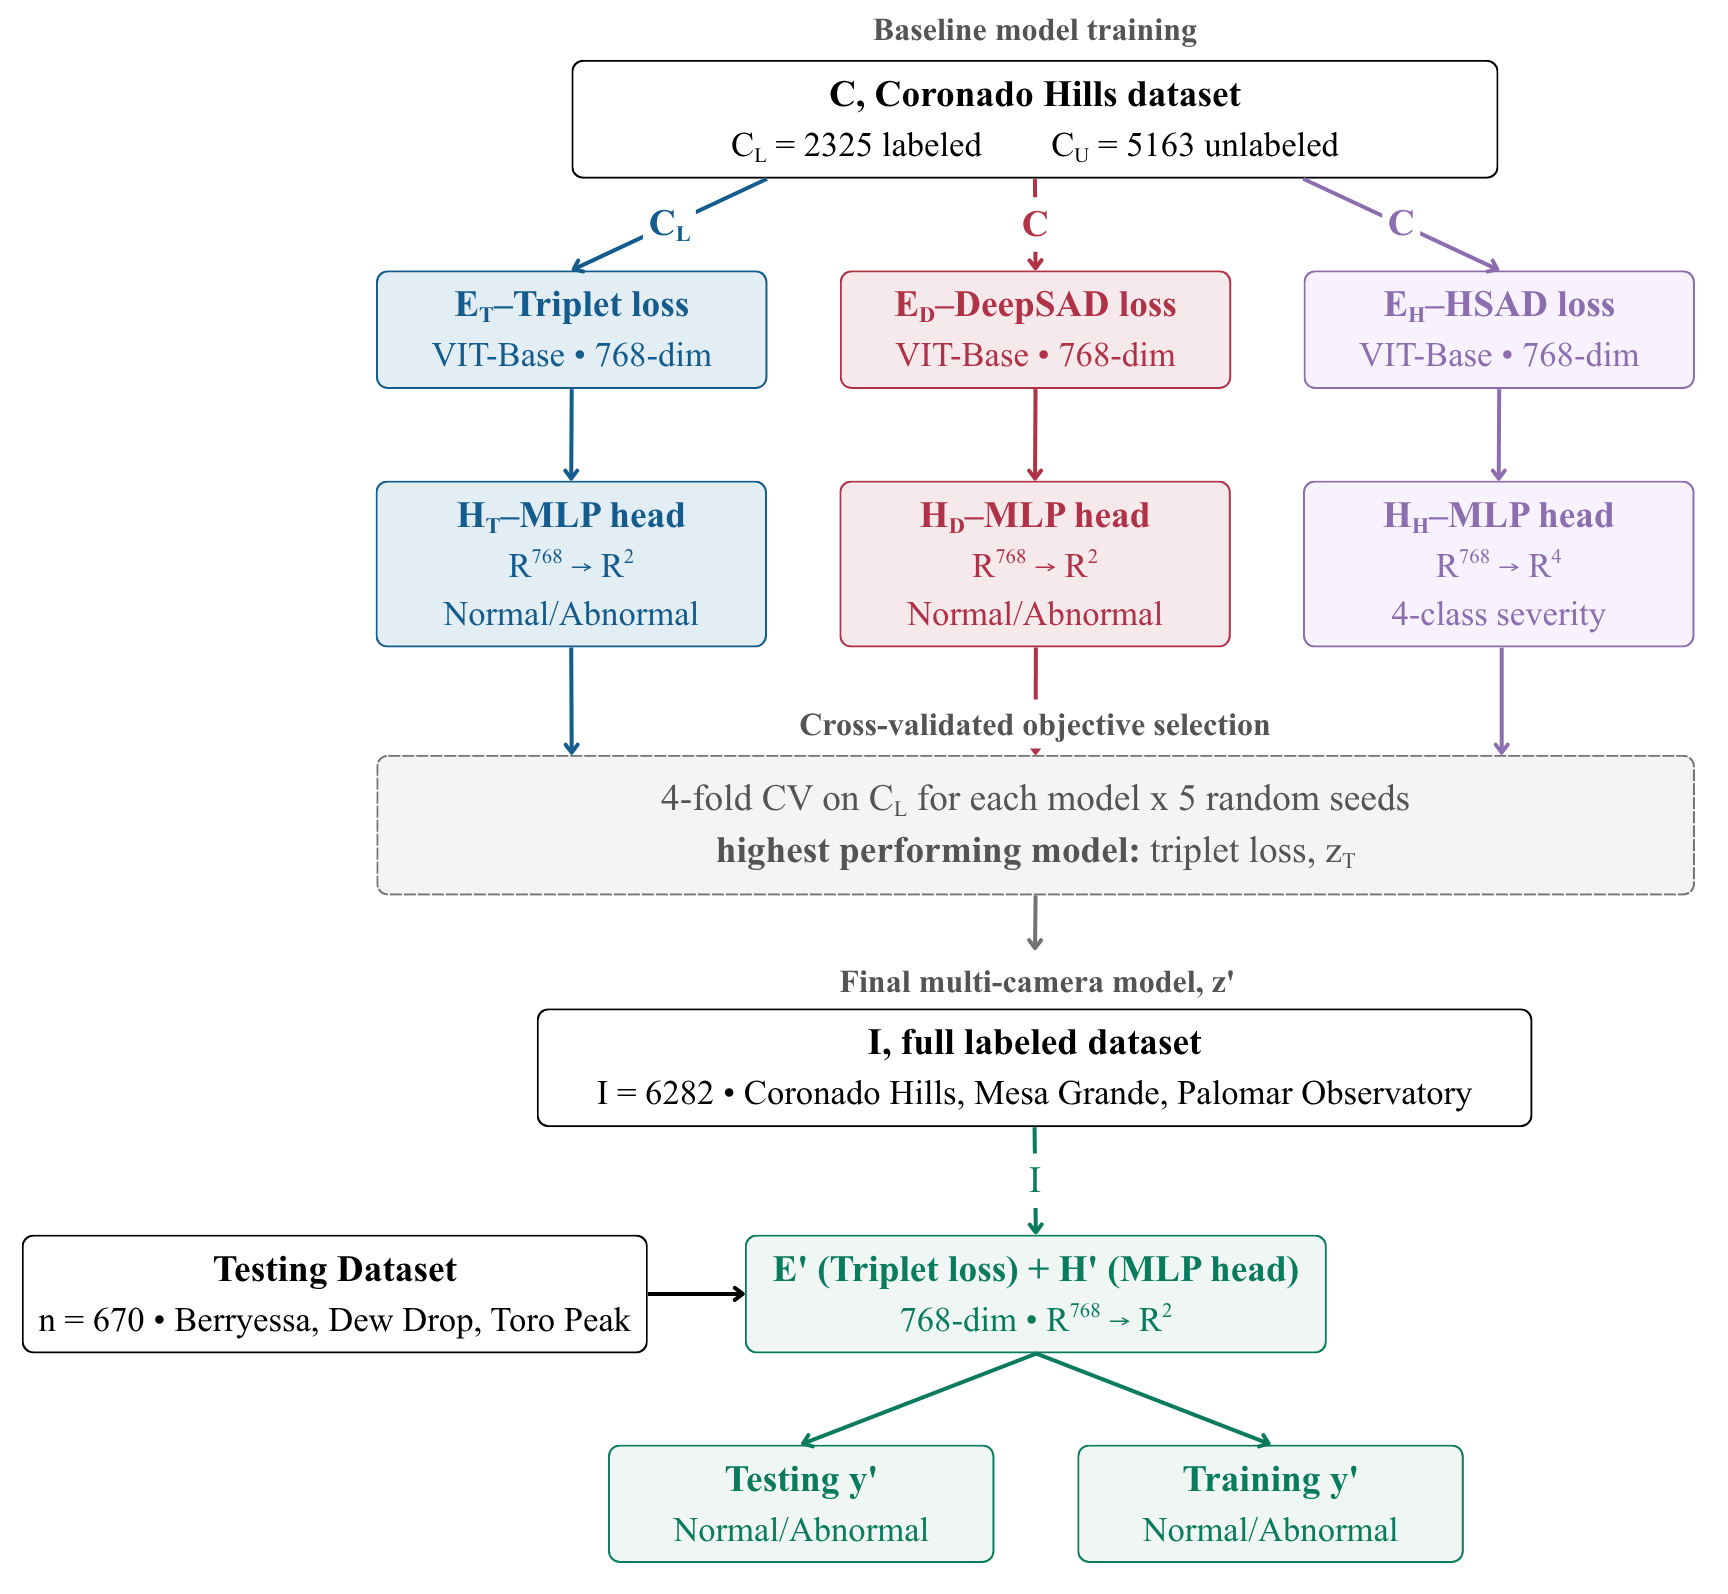
\includegraphics[width=0.85\linewidth]{figures/model_pipeline.png}
    \caption{Flowchart outlining the full training pipeline of the model, from baseline models to the final multi-camera model.}
    \label{fig:model_pipeline}
\end{figure}

\subsection{Data Collection and Preprocessing}
\label{sec:datacollection}

We source the data from cameras in the ALERTCalifornia network. These cameras exhibit variations in weather conditions, lighting, and terrain (as seen in Figure~\ref{fig:level_examples}), making them suitable for training and testing the \Ac{QoS} anomaly detection model. To construct the labeled dataset, we extract still images from cameras over a one-year period: October 1, 2024, to September 30, 2025. We sample frames at a fixed hourly interval by selecting the image closest to the top of each hour. Because camera views may occasionally be adjusted by local emergency operators, we use pan, tilt, and zoom information from the external metadata to maintain visual consistency across the dataset. Specifically, we exclude frames whose values deviate from the camera-specific median by more than 4° in pan, 0.1° in tilt, or 0.1x in zoom. These thresholds are chosen to minimize scene variation across cameras during model training. Table~\ref{tab:frame_counts} describes the size of each dataset after filtering. 
\begin{table}[H]
\scriptsize
\centering
\begin{threeparttable}

\caption{Counts of frames from each camera location across training and testing sets.}
\label{tab:frame_counts}

\begin{tabular}{@{}lrrrr@{}}
\toprule
\multicolumn{5}{c}{\textbf{Training Data}} \\
\midrule
& Coronado Hills & Mesa Grande & Palomar Observatory$^{*}$ & Total \\
\midrule

Level 1-Clear  & 977  & 1367 & 1271 & 3615 \\
Level 2-Minor  & 813  & 217  & 363  & 1393 \\
\textbf{Normal}  & 1790 & 1584 & 1634 & 5008 \\

\midrule
Level 3-Major  & 226  & 91  & 254  & 571 \\
Level 4-Severe & 309  & 240 & 153  & 702 \\
\textbf{Abnormal}& 535  & 331  & 407  & 1273 \\

\midrule
\textbf{Labeled}   & 2325 & 1915 & 2041 & 6281 \\
\textbf{Unlabeled} & 5163 & 6003 & 4822 & 15988 \\

\midrule
\textbf{Total} & 7488 & 7918 & 6863 & 22269 \\
\bottomrule

\addlinespace[0.5em]

\toprule
\multicolumn{5}{c}{\textbf{Testing Data}} \\
\midrule
& Toro Peak$^{*}$ & Dew Drop$^{*}$ & Berryessa & Total \\
\midrule

Level 1 - Clear  & 155 & 143 & 110 & 408 \\
Level 2 - Minor  & 60  & 38  & 49  & 147 \\
\textbf{Normal}  & 215 & 181 & 159 & 555 \\

\midrule
Level 3 - Major  & 26 & 24 & 9 & 59 \\
Level 4 - Severe & 15 & 7 & 34 & 56 \\
\textbf{Abnormal}& 41 & 31 & 43 & 115 \\

\midrule
\textbf{Labeled}   & 256 & 212 & 202 & 670 \\
\textbf{Unlabeled} & 7167 & 7777 & 6947 & 21891 \\

\midrule
\textbf{Total} & 7423 & 7989 & 7149 & 22561 \\
\bottomrule
\end{tabular}

\begin{tablenotes}
\footnotesize
\item[*]Seasonal camera locations. These cameras exhibit substantial environmental variation throughout the year.
\end{tablenotes}

\end{threeparttable}
\end{table}


To train our initial model, we focus on three cameras located in San Diego County: Axis-CoronadoHillsS \footnote{\url{https://cameras.alertcalifornia.org/?id=Axis-CoronadoHillsS}}, Axis-PalomarObs1 \footnote{\url{https://cameras.alertcalifornia.org/?id=Axis-PalomarObs1}}, and Axis-MesaGrandeNorth \footnote{\url{https://cameras.alertcalifornia.org/?id=Axis-MesaGrandeNorth}}. Throughout the rest of this paper, we will refer to these three locations as Coronado Hills, Palomar Observatory, and Mesa Grande, respectively. These cameras capture different landscapes and varying degrees of seasonal change, making them suitable for our objective. Specifically, Coronado Hills and Mesa Grande demonstrate consistent views across seasons. Palomar Observatory captures notable seasonal changes, such as snow, ice, and changes in foliage color. This variety provides extra flexibility to control for seasonal effects in our model. 

In the testing set, we introduce three additional cameras: Axis-ToroPeak1 \footnote{\url{https://cameras.alertcalifornia.org/?id=Axis-ToroPeak1}}, Axis-Dewdrop1 \footnote{\url{https://cameras.alertcalifornia.org/?id=Axis-Dewdrop1}}, and Axis-Berryessa \footnote{\url{https://cameras.alertcalifornia.org/?id=Axis-Berryessa}}, which we refer to as Toro Peak, Dew Drop, and Berryessa. In this set, Toro Peak and Dew Drop are seasonal cameras, while Berryessa does not show substantial change across seasons. We select Dew Drop and Berryessa, located in Amador and Yolo Counties in Northern California, to evaluate the model's ability to generalize across geographic regions. Toro Peak, also located in Southern California in Riverside County, is selected to assess seasonal effects in a similar area. This configuration allows us to evaluate model performance across both seasonal variability and geographic context. Example images from each location are shown in Figure~\ref{fig:level_examples}. 

\begin{figure}[H]
    \centering
    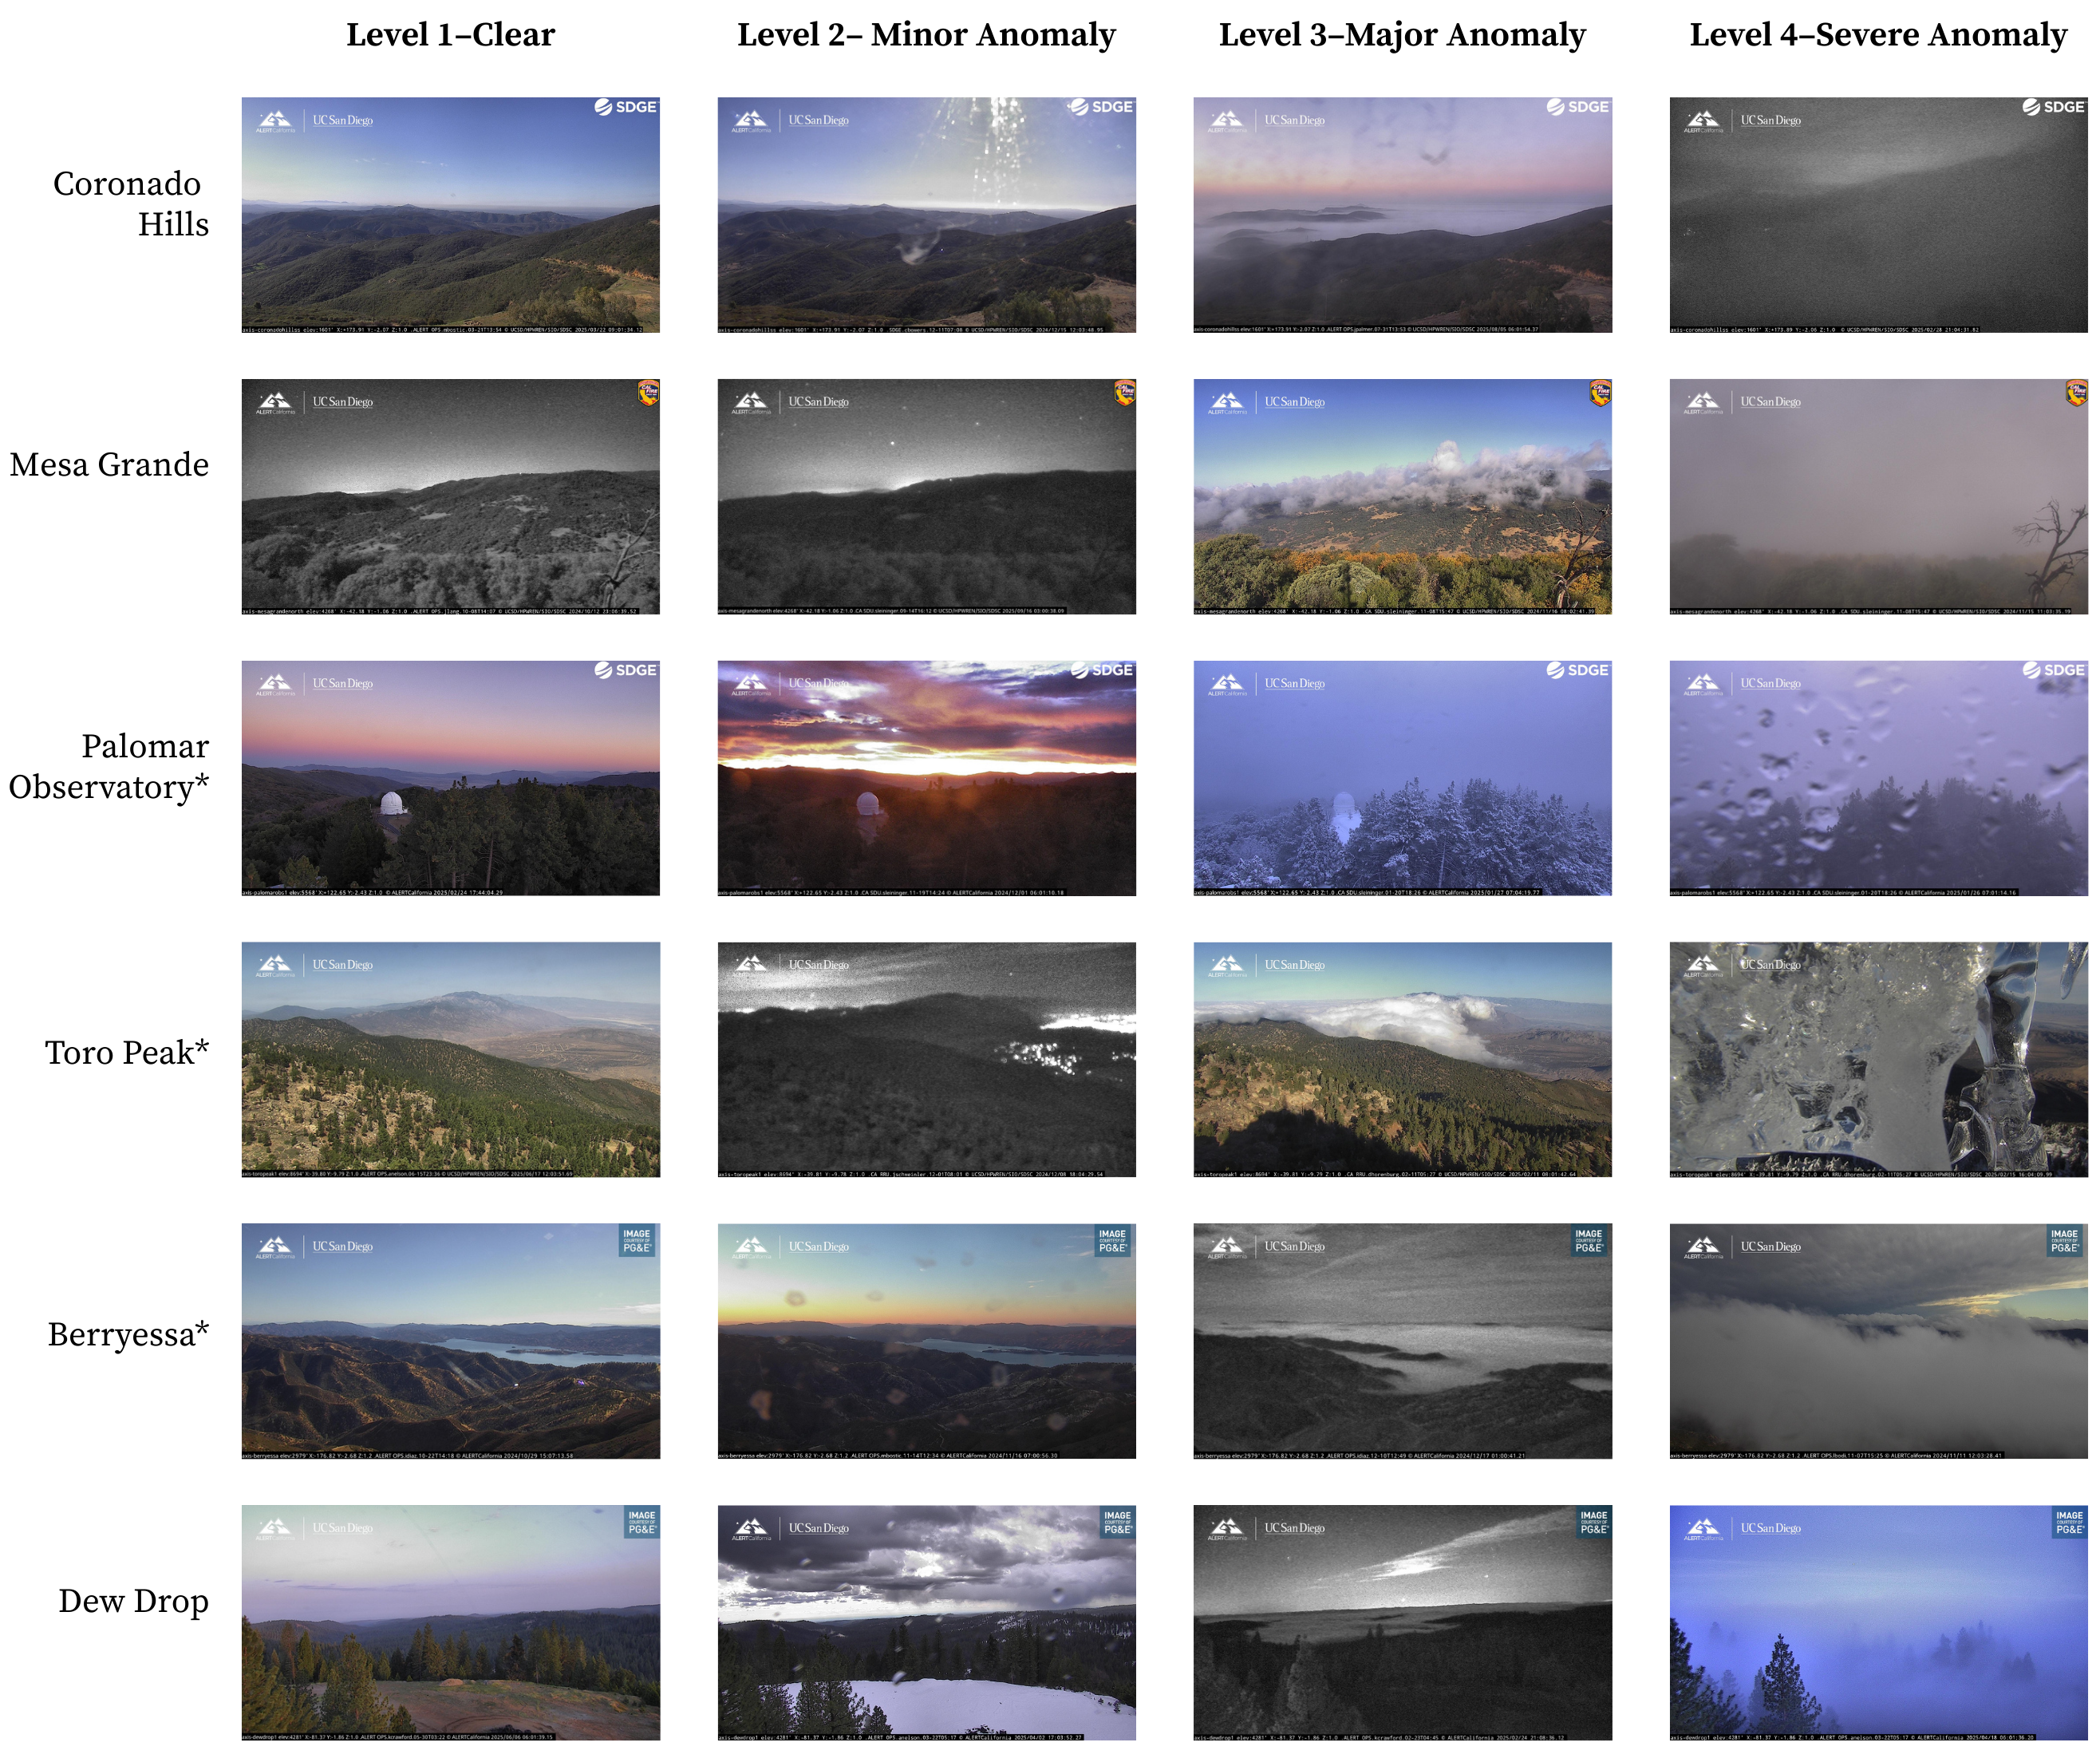
\includegraphics[width=1\linewidth]{figures/level_image_grid.png}
    \caption{Representative frames corresponding to each level of the 4-point ordinal scale across all six cameras. Camera locations ordered from top to bottom: Coronado Hills, Mesa Grande, Palomar Observatory, Toro Peak, Berryessa, Dew Drop.}
    \label{fig:level_examples}
\end{figure}

\subsection{Label Definition and Annotation}
\label{sec:datalabeling}

To construct our labeled dataset for supervised learning, we design a camera-agnostic labeling scheme with a strict rubric to enhance consistency across four annotators. The 4-point ordinal scale is outlined as follows. We define the \ac{ORR} of an image as the non-sky portion that contains terrain, infrastructure, and other elements critical to response operations.

\begin{itemize}
    \item\textbf{Level 1-Clear:} Normal operation of the camera with no observable obstruction or quality issues. The camera is fully reliable for response operations.
    \item\textbf{Level 2-Minor:} Translucent obstructions (\textless 50\% of the \ac{ORR}) cause partial obstruction of the camera's field of view. The camera remains reliable for response operations.
    \item\textbf{Level 3-Major:} Opaque obstructions (\textgreater 50\% of the \ac{ORR}) cause partial obstruction of the camera's field of view. The camera may not be reliable for response operations.
    \item\textbf{Level 4-Severe:} An obstruction covers \textgreater 50\% of the \ac{ORR}. The camera is unreliable for response operations.                   
\end{itemize}

Four annotators review each image to ensure labeling consistency and reduce subjective bias. The final label is determined by majority opinion, in which at least 3 annotators agree. Images with conflicting or tied labels are separately addressed in a team meeting to reach a consensus. To assess inter-rater agreement, we compute Krippendorff's $\alpha$ using the ordinal severity labels, obtaining a value of 0.6939. Leveraging Label Studio's random sampling setting, we complete a total of 6,281 tasks for the training set (see Table~\ref{tab:frame_counts} for complete counts). Figure~\ref{fig:level_examples} highlights examples of each level across cameras using this labeling scheme. 

Once we obtain our labeled dataset, we downsample and standardize the images to a size of 224 x 224 pixels with 3 channels. Then, we convert them into tensors of size 224 x 224 x 3. In their processed form, each image has 150,528 features.  We then partition the dataset collected from the three training cameras into a random 80\% training and a 20\% held-out test split. This training split is used to optimize the model, while the held-out test split provides an evaluation on unseen images from the same camera locations. Finally, all training and held-out test data are divided into batches of size 32 to maximize the computational power of a single \ac{GPU} during training. 

\subsection{Model Training}

Our training process can be divided into two phases: \textbf{objective selection} and \textbf{multi-camera training}. 

During objective selection, we evaluate the effectiveness of different training objectives on a single camera. We train three baseline models using three different loss functions: triplet margin loss (see Appendix~\ref{app:marginloss}), \ac{DeepSAD} loss (see Appendix~\ref{app:deepsad}), and \ac{H-SAD} loss (see Appendix~\ref{app:hsad}). Triplet margin loss is a supervised objective, while \ac{DeepSAD} and \ac{H-SAD} are semi-supervised objectives. 

To ensure robust evaluation, we implement a stratified 4-fold cross-validation framework. The training set is partitioned into four folds using random stratified sampling based on class labels so that each fold has a representative distribution of class labels. During each iteration, three folds are used for training, while the final fold is held out as the validation set. 

During each iteration, we train a two-stage pipeline consisting of an encoder and a classification head. The encoder is trained only on the training folds, after which embeddings are computed for both training and validation partitions. The classification head is then trained exclusively on the training embeddings and evaluated on the corresponding validation embeddings. We measure model performance using classification accuracy, precision, and recall for both sets. After completing all cross-validation iterations, we compute the mean and \ac{SD} of metrics across validation folds. 

We refer to the models trained using triplet loss, \ac{DeepSAD} loss, and \ac{H-SAD} loss as $\mathbf{z_T}$,  $\mathbf{z_D}$, and $\mathbf{z_H}$, respectively. Each model takes a set of processed images as input and outputs a predicted \ac{QoS} label, although the dimensionality varies across objectives. Specifically, for $\mathbf{z_T}$ and $\mathbf{z_D}$, we formulate the task as a binary classification problem where we group Clear and Minor under a single Normal class, and Major and Severe under a single Abnormal class. This structure reflects the operational significance of the anomalies, as Clear and Minor frames generally do not require immediate attention, whereas Major and Severe anomalies may substantially impair image reliability and camera utility. 

In contrast, $\mathbf{z_H}$ is trained using the original four-level severity annotation scheme as the objective was specifically designed for the ranked relationship of these classes. This allows us to evaluate whether preserving finer severity information improves detection performance relative to the binary design. All models are trained exclusively using images from the Coronado Hills camera. 

\subsubsection{Model Architecture}
\label{sec:architecture}

We separate each model $\mathbf{z_i} \in \{\mathbf{z_T}, \mathbf{z_D}, \mathbf{z_H}\}$ into two components: the encoder $\mathbf{E_i} \in \{\mathbf{E_T}, \mathbf{E_D}, \mathbf{E_H}\}$ and the classification head $\mathbf{H_i} \in \{\mathbf{H_T}, \mathbf{H_D}, \mathbf{H_H}\}$ (refer to Figure~\ref{fig:model_pipeline} for the full model pipeline). The processed images are first passed through the encoder, which outputs an embedding for each image. These embeddings are then passed into the classification head, which subsequently returns a classification label for each. The relationships can be written as follows, where $x$ is a set of processed images:
\[\mathbf{z_i}(x) = \mathbf{H_i}(\mathbf{E_i}(x))\] 

Each encoder $\mathbf{E_i}$ utilizes a \ac{ViT} architecture to map input images into a lower-dimensional feature space. We initialize all encoders using publicly available ViT-Base weights pretrained on ImageNet-21k and fine-tuned on ILSVRC-2012 \cite{deng2009imagenet, wu2020visual}. By default, a ViT (as implemented by Dosovitskiy et al.) consists of patch embedding, position embedding, transformer encoder, and \ac{MLP} classification head segments (Figure~\ref{fig:vit_model}). We modify our encoder's architecture by removing the \ac{MLP} classification head (shown in the top orange box in Figure~\ref{fig:vit_model}), so that its outputs come directly from the transformer encoder layer. All outputs are 768-dimensional, and all encoders share an identical architecture; they differ only in the values of their weights. 

\begin{figure}[H]
    \centering
    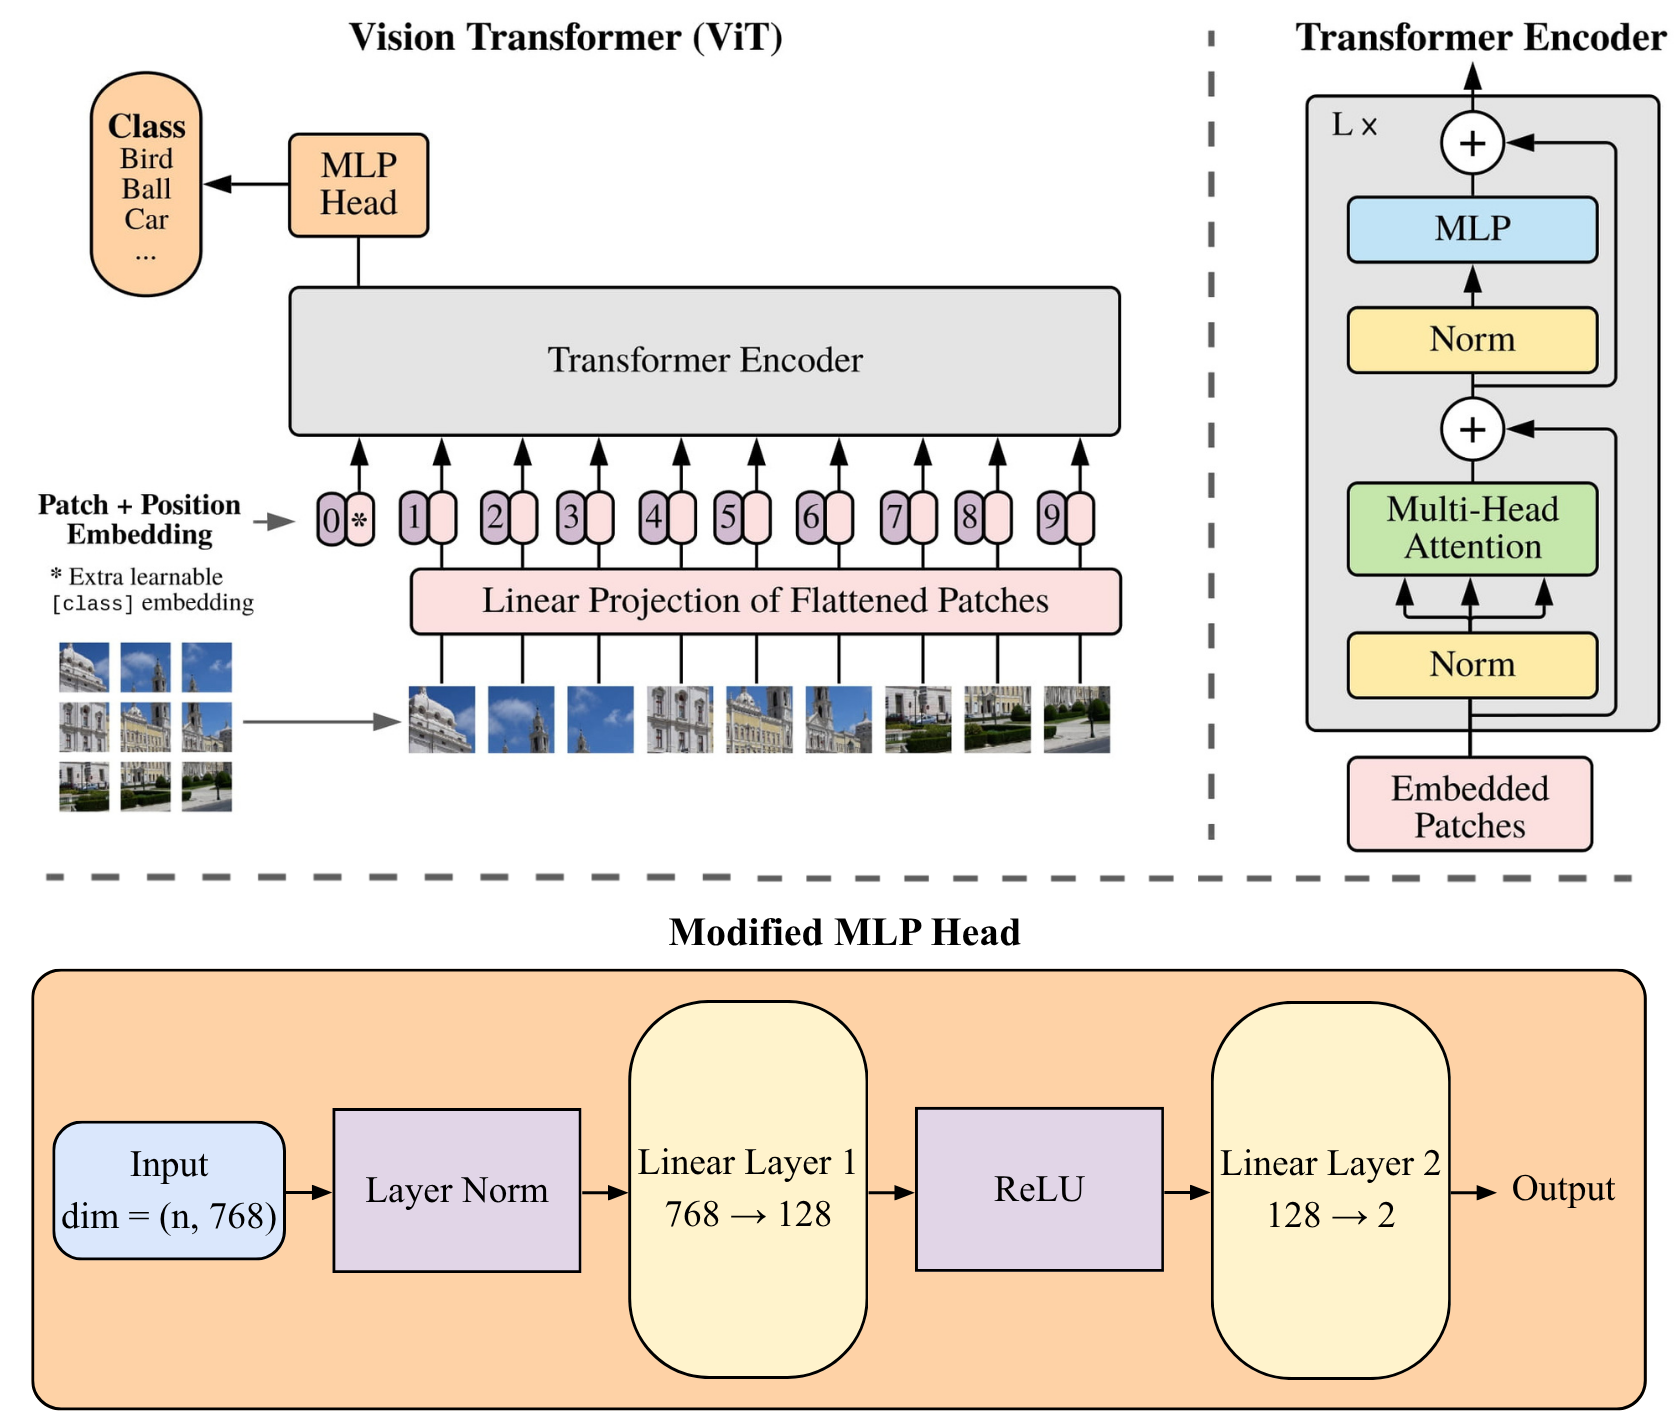
\includegraphics[width=0.9\linewidth]{figures/vit_model.png}
    \caption{Overview of the Vision Transformer (ViT) architecture \cite{dosovitskiy2021an}. Input images are split into patches, embedded, and processed through a transformer encoder. In our framework, the original MLP classification head is removed, and a separate MLP head is applied to the resulting embeddings for anomaly classification.}
    \label{fig:vit_model}
\end{figure}

To perform classification, we introduce a separate \ac{MLP} head $\mathbf{H_i} \in \{\mathbf{H_T}, \mathbf{H_D}, \mathbf{H_H}\}$, illustrated in orange at the bottom of Figure~\ref{fig:vit_model}. Each head consists of two layers with a ReLU nonlinearity. The key difference from the original \ac{ViT} implementation is the addition of a layer norm function and a second linear layer. These add more depth to the network, allowing it to capture more complex relationships between features. Each model returns either two or four-dimensional outputs corresponding to the class labels they are trained on. 

\subsubsection{Objective Selection}

We first train each of $\mathbf{E_i} \in \{\mathbf{E_T}, \mathbf{E_D}, \mathbf{E_H}\}$ separately, each with its own objective function. $\mathbf{E_T}$ is trained exclusively on the labeled Coronado Hills dataset, while $\mathbf{E_D}$ and $\mathbf{E_H}$ are trained using both labeled and unlabeled Coronado Hills data. $\mathbf{E_T}$ is trained using triplet margin loss, $\mathbf{E_D}$ is trained using \ac{DeepSAD} loss, and $\mathbf{E_H}$ is trained using \ac{H-SAD} loss. The various hyperparameters used for each objective are outlined in Table~\ref{tab:hyperparams}. These hyperparameters yield the best separation between classes in the embedding space. Additionally, we utilize hard negative mining while training $\mathbf{E_T}$ to optimize the learning process (see Appendix~\ref{app:mining}). Through this process, we obtain baseline encoders to analyze our data.

\begin{table}[H]
\centering

\caption{Hyperparameters used for training each encoder.}
\label{tab:hyperparams}

\begin{tabular}{lcccccc}
\toprule
\textbf{Encoder} & \textbf{Margin} & $\boldsymbol{\eta}$ & $\boldsymbol{\alpha}$ & $\boldsymbol{\lambda}$ & \textbf{Learning rate} & \textbf{Epochs} \\
\midrule

$\mathbf{E_T}$ & $1.9 \times 10^{-1}$ & -- & -- & -- & $1 \times 10^{-5}$ & 10 \\
$\mathbf{E_D}$ & -- & $1 \times 10^{1}$ & -- & $1 \times 10^{-7}$ & $1 \times 10^{-6}$ & 1 \\
$\mathbf{E_H}$ & -- & $1 \times 10^{-2}$ & $1 \times 10^{1}$ & $1 \times 10^{-6}$ & $1 \times 10^{-5}$ & 5 \\

\bottomrule
\end{tabular}

\end{table}


After training each encoder, we obtain three sets of embeddings, $\mathbf{e_i} \in  \{\mathbf{e_T}, \mathbf{e_D}, \mathbf{e_H}\}$, by running inference on the labeled Coronado Hills data, $\mathbf{C_L}$. Since the classification head is trained with a supervised objective, we run inference only on the labeled dataset. 

Finally, we separate each image embedding set into batches of size 32 and use each to train its corresponding \ac{MLP} head $\mathbf{H_i} \in \{\mathbf{H_T}, \mathbf{H_D}, \mathbf{H_H}\}$. For simplicity, we train using the cross-entropy loss function, as provided by PyTorch \footnote{\url{https://pytorch.org/}}. By using each $\mathbf{H_i}$ to perform inference on its corresponding embedding, we obtain output sets $\mathbf{y_i} \in \{\mathbf{y_T}, \mathbf{y_D}, \mathbf{y_H}\}$, where:
%\[\left|\mathbf{y_T}\right| = \left|\mathbf{y_D}\right| = \left|\mathbf{y_H}\right| =X\]
\[\mathbf{y_T} \in \mathbb{R}^2, \quad \mathbf{y_D} \in \mathbb{R}^2, \quad\mathbf{y_H} \in \mathbb{R}^4\]

Each $\mathbf{y_i}$ can be used to compute a classification for each image in $\mathbf{C_L}$. $\mathbf{y_T}$ and $\mathbf{y_D}$ yield classifications of Normal or Abnormal, while $\mathbf{y_H}$ yields a classification of Clear, Minor, Major, or Severe. Using these outputs, we analyze each model to determine which objective function to move forward with for multi-camera training. The results of this analysis can be found in Section~\ref{sec:results}.

\subsubsection{Multi-Camera Training}

Through evaluation of classification accuracies, our analysis determined the optimal objective function to be the triplet margin loss. Thus, for our final model, we construct a model $\mathbf{z'}$, consisting of components $\mathbf{E'}$ and $\mathbf{H'}$.

We first train $\mathbf{E'}$ on the full set of labeled training data across all three cameras—Coronado Hills, Palomar Observatory, and Mesa Grande—denoted as $\mathbf{I}$. For the hyperparameters, we choose a margin of 0.19 and train for 10 epochs, as these parameters yield the best separation between Normal and Abnormal points in the embedding space. Once this is complete, we obtain a set of embeddings. 

Finally, we train $\mathbf{H'}$ on $\mathbf{I}$ using the same cross-entropy loss function used during objective selection. The outputs returned by $\mathbf{H'}$ are two-dimensional and classify points as Normal or Abnormal.

%%%%%%%%%%%%%%%%%%%%%%%%%%%%%%%%%%%%%%%%%%
\section{Results}
\label{sec:results}

\subsection{Baseline Models}
In our objective selection process, we train and evaluate each baseline model on the Coronado Hills dataset using 4-fold cross-validation. For each model, we take the mean and standard deviation of training and validation accuracies across folds. We then repeat this process using five randomly selected training seeds and record the average mean and standard deviation. Table~\ref{tab:train_val_accs} summarizes the results of this analysis. Overall, across three objective functions, triplet loss consistently outperforms \ac{DeepSAD} and \ac{H-SAD} in both training and validation sets. 

\begin{table}[H]
\centering

\caption{Training and validation accuracies for each baseline model. The average mean training accuracy is calculated across 5 seeds, each with 4-fold cross-validation.}
\label{tab:train_val_accs}

\begin{tabular}{lccc}
\toprule
\textbf{Metric} & $\mathbf{z_T}$ & $\mathbf{z_D}$ & $\mathbf{z_H}$ \\
\midrule

Average mean training accuracy & 0.9979 & 0.9348 & 0.7227 \\
Average training SD & 0.0015 & 0.0062 & 0.0316 \\
Average mean validation accuracy & 0.9260 & 0.9094 & 0.6903 \\
Average validation SD & 0.0105 & 0.0177 & 0.0300 \\

\bottomrule
\end{tabular}

\end{table}

\subsection{Final Multi-Camera Model}

We adopt triplet loss in our final model architecture due to its superior performance in baseline evaluations. The final multi-camera model is trained on data from Coronado Hills, Palomar Observatory, and Mesa Grande. We further assess intra-dataset performance by evaluating the model on a held-out test set that includes unseen samples from these three locations. Because the distribution of camera frames is imbalanced and skewed towards Normal, we report the balanced accuracy in addition to standard classification metrics. Table~\ref{tab:train_test_accs} presents the results. 
\begin{table}[H]
\centering

\caption{Final model performance on training and held-out test.}
\label{tab:train_test_accs}

\begin{tabular}{lcccc}
\toprule
\textbf{Metric} & \begin{tabular}[c]{@{}c@{}}Coronado\\Hills\end{tabular} & \begin{tabular}[c]{@{}c@{}}Mesa\\Grande\end{tabular} & \begin{tabular}[c]{@{}c@{}}Palomar\\Observatory$^{*}$\end{tabular} & Average  \\
\midrule

Training balanced accuracy & 0.9980 & 1.0000 & 0.9959 & 0.9980 \\
Test balanced accuracy    & 0.9183 & 0.9530 & 0.9276 & 0.9329 \\
Test recall       & 0.8505 & 0.9091 & 0.8765 & 0.8787 \\
Test precision    & 0.9479 & 0.9836 & 0.9103 & 0.9472 \\

\bottomrule
\end{tabular}

\vspace{4pt}
\footnotesize
$^{*}$Seasonal camera locations.

\end{table}

Training balanced accuracy is near-perfect across all three locations, whereas test balanced accuracy remains in the 90\% range. Recall, which measures the model's ability to correctly identify all \ac{QoS} anomalies, is overall lower than precision, which measures the proportion of correctly predicted anomalies. 

\subsection{Generalization Across Camera Locations}
% To assess the model's potential to generalize, we examine learned embeddings in the PC1 and PC2 space. Figure~\ref{fig:final_pc_proj} displays the projection, where each point corresponds to a single image in the dataset and is colored according to its associated camera location. The embeddings are computed from the final trained encoder and projected into two dimensions using \ac{PCA}. This visualization directly compares spatial representations across camera sites. 

% \begin{figure}[H]
%     \centering
%     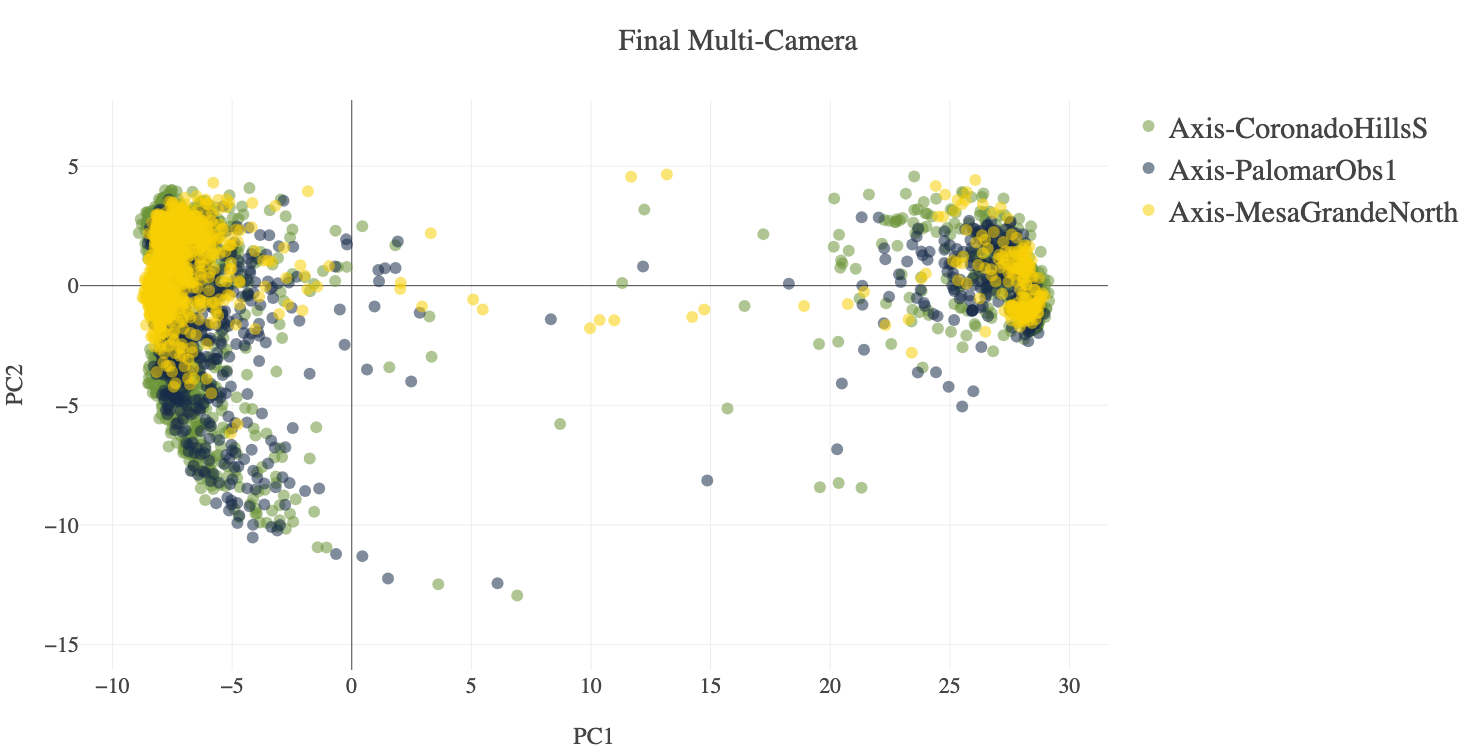
\includegraphics[width=0.85\linewidth]{figures/final_p1p2.png}
%     \caption{PC1 vs. PC2 projection of the final model trained using triplet loss, colored by
% camera locations.}
%     \label{fig:final_pc_proj}
% \end{figure}

We test generalization beyond the training distribution by evaluating on three new unseen datasets: Berryessa, Dew Drop, and Toro Peak. Table~\ref{tab:camera_accuracies} lists the balanced accuracy, precision, and recall values. 

\begin{table}[H]
\centering

\caption{Performance on unseen camera test set.}
\label{tab:camera_accuracies}

\begin{tabular}{lcccc}
\toprule
\textbf{Metric} & Berryessa & Dew Drop$^{*}$ & Toro Peak$^{*}$ & Average \\
\midrule

Balanced accuracy & 0.7431 & 0.9061 & 0.8373 & 0.8288 \\
Precision & 0.3500 & 0.4769 & 0.5410 & 0.4560 \\
Recall & 0.9767 & 1.000 & 0.8049 & 0.9272 \\

\bottomrule
\end{tabular}

\vspace{4pt}
\footnotesize
$^{*}$Seasonal camera locations.

\end{table}

To further assess the model's performance independent of a specific decision threshold, we generate \ac{PRC} curves and the corresponding \ac{AUPRC} for each camera location in Figure~\ref{fig:roc_curves}. These curves characterize the tradeoff between precision and recall across all possible decision thresholds, providing additional insight into the model's ability to distinguish with an imbalanced dataset. 

%%%%%%%%%%%%%%%%%%%%%%%%%%%%%%%%%%%%%%%%%%
\section{Discussion}

The results demonstrate that embedding-based anomaly detection can effectively identify image quality degradations. In this section, we discuss the key takeaways from the final model performance and analyze the final model's performance with respect to both in-distribution generalization (held-out test set) and out-of-distribution generalization across unseen camera locations. We also discuss the key limitations of our proposed approach and outline directions for future work. 

\subsection{Baseline Models}
Across the cross-validation folds, triplet loss achieves the highest validation accuracy ($92.60 \pm 1.05\%$), followed by \ac{DeepSAD} ($90.94 \pm 1.77\%$) and \ac{H-SAD} ($69.03 \pm 3.00\%$). It also demonstrates the most consistent results, with the lowest standard deviations across all training and validation tests. Both triplet loss and \ac{DeepSAD} achieve accuracies in the $90\%$ range while \ac{H-SAD} is the only objective function failing to meet that threshold. The large gap between \ac{H-SAD} and its alternatives likely reflects differences in label structure, in which the former is trained using a 4-point severity scale while the latter are trained using binary Normal/Abnormal labels. As such, learning more levels requires capturing more nuanced ordinal distinctions in image quality degradation, which can make the classification task inherently more difficult. 

\subsection{Final Multi-Camera Model}
The final multi-camera model trained with triplet loss demonstrates relatively strong performance across all three camera locations in the training distribution. As shown in Table~\ref{tab:train_test_accs}, held-out balanced accuracies exceed 90\% at every location, indicating that the model generalizes effectively to previously unseen samples drawn from familiar environmental conditions. Across all three cameras, precision consistently exceeds recall, suggesting that the model adopts a more conservative approach that favors detection accuracy over missed events. Although this strategy results in some missed \ac{QoS} anomalies, it also reduces the number of false alarms. 

\subsection{Generalization Across Camera Locations}
% The embedding projection onto the shared latent space defined by PC1 and PC2 reveals that all camera locations occupy overlapping regions, though with varying degrees of dispersion (Figure~\ref{fig:final_pc_proj}). While some location-dependent spread is observed, there appears to be no distinct clusters corresponding to individual cameras. This suggests that the dominant variation captured by the learned representations is not solely driven by camera identity. This behavior is encouraging for generalization, as the absence of camera-specific outliers indicates that embeddings learned from different locations largely share a feature space. 

For unseen cameras, classification accuracies reported in Table~\ref{tab:camera_accuracies} indicate an average balanced accuracy of 82.88\%. However, accuracy alone does not fully capture model performance, and in this setting, it hides a significant tradeoff between precision and recall. In particular, across all unseen locations, the model achieves a high average recall of 92.72\% but a considerably lower precision of 45.60\%, suggesting a tendency to over-predict \ac{QoS} anomalies. As a result, the model successfully identifies most of the anomalous frames at the expense of more false positives. This behavior is opposite to that observed in the training distribution and indicates that the model becomes less conservative when presented with new camera locations. Instead, the model shifts to adopt a sensitivity-focused approach that prioritizes detection coverage over minimizing false alarms. In the context of environmental monitoring, however, this tradeoff may be acceptable, as the consequence of missing a \ac{QoS} event can be greater than the cost of reviewing a false alarm. 

Despite the reduction in precision, Figure~\ref{fig:roc_curves} shows that all camera locations achieve \ac{AUPRC} values above 0.68, substantially exceeding their positive-class baselines of 0.1462 to 0.2129. These results indicate that the model effectively separates Abnormal frames from Normal frames, even under class imbalance. The discrepancy between the \ac{AUPRC} values and lower precision suggests that classification accuracies may be more sensitive to the selected decision threshold, and that the model's anomalous discrimination remains reliable. Current results reflect a default decision threshold that favors recall over precision, rather than an inability to distinguish between normal and anomalous frames. 

Performance also varies across individual camera locations within the unseen dataset. Interestingly, Dew Drop and Toro Peak, both identified as seasonal cameras, outperform Berryessa, a location that does not observe significant seasonal variability. Dew Drop and Toro Peak achieve balanced accuracies of 90.61\% and 83.73\%, respectively, compared to Berryessa's 74.31\%. These results suggest that rather than seasonal factors, the model's ability to generalize is more heavily influenced by other environmental characteristics. In particular, Toro Peak, which is located in Southern California and shares visual characteristics with the training distribution, achieves the highest balanced accuracy and precision among the three unseen locations. Unlike Berryessa and Dew Drop, it does not exhibit the pronounced imbalance between precision and recall, indicating a more stable tradeoff between false positives and false negatives. Overall, these results suggest that the model generalizes more effectively to camera locations whose visual characteristics resemble those seen in training. 

\begin{figure}[H]
    \centering

    % ================= Row 1 =================
    \subfloat[Coronado Hills]{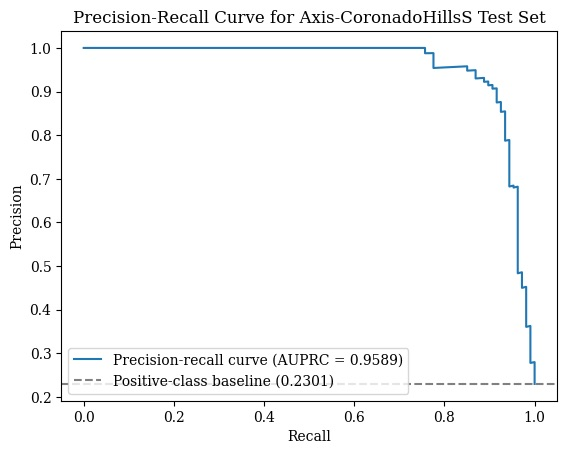
\includegraphics[width=0.48\textwidth]{figures/coronado_hills_prc.png}}
    \hfill
    \subfloat[Mesa Grande]{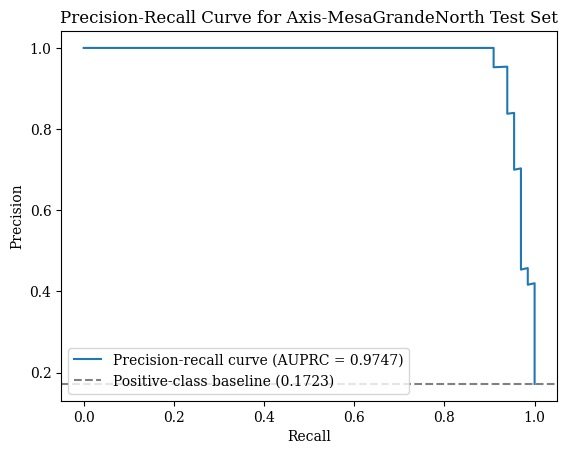
\includegraphics[width=0.48\textwidth]{figures/mesa_grande_prc.png}}

    \vspace{0.4cm}

    % ================= Row 2 =================
    \subfloat[Palomar Observatory]{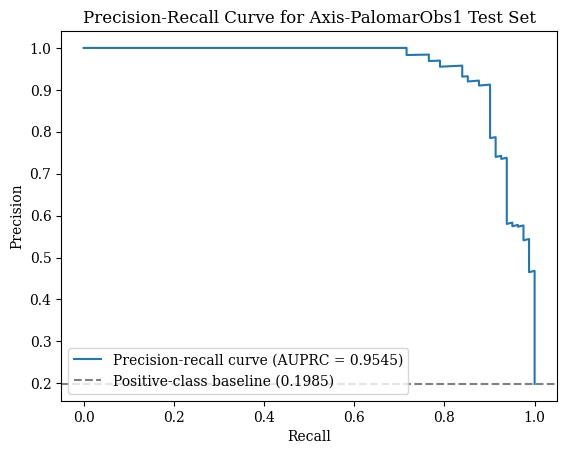
\includegraphics[width=0.48\textwidth]{figures/palomar_prc.png}}
    \hfill
    \subfloat[Berryessa]{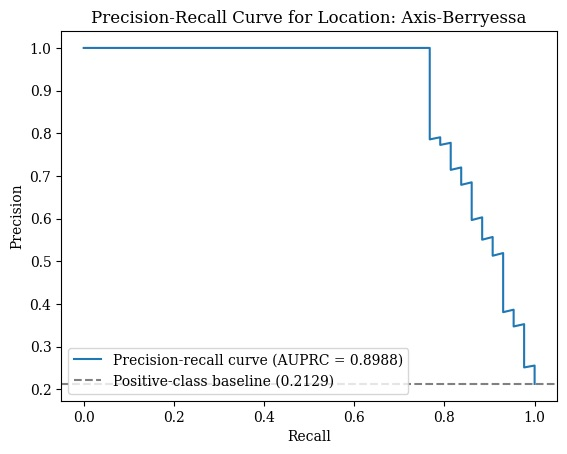
\includegraphics[width=0.48\textwidth]{figures/berryessa_prc.png}}

    \vspace{0.4cm}

    % ================= Row 3 =================
    \subfloat[Dew Drop]{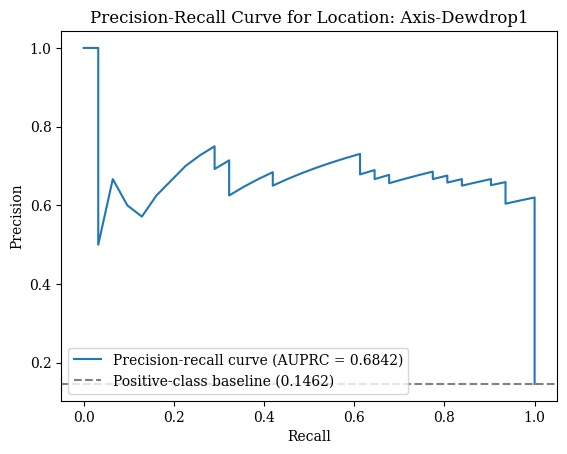
\includegraphics[width=0.48\textwidth]{figures/dewdrop_prc.png}}
    \hfill
    \subfloat[Toro Peak]{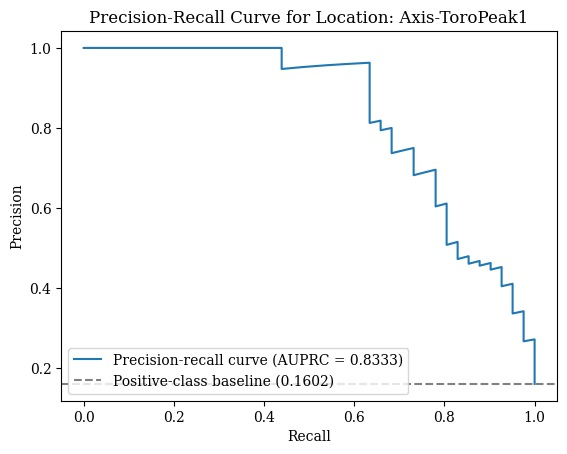
\includegraphics[width=0.48\textwidth]{figures/toropeak_prc.png}}

    \caption{Precision-recall curves and \ac{AUPRC} across all camera locations for held-out (a-c) and unseen (d-f) camera test sets.}
    \label{fig:roc_curves}
\end{figure}

\subsection{Analysis of False Positive Frames}

This trend becomes even more apparent when examining false positive frames from the unseen camera locations, as seen in Figure~\ref{fig:false_positives}. Unlike all other cameras, Berryessa contains a large body of water, which is a visual feature unique to its location. Especially during low light conditions, this water surface resembles a layer of cloud (see Figure~\ref{fig:false_positives}). We hypothesize that this feature likely explains the disproportionately large number of false positives, as it mirrors visual cues that the model associates with \ac{QoS} anomalies. These findings reinforce that the model is capable of generalizing across seasonal and environmental variation when the visual characteristics remain similar to those seen during training. However, performance declines when novel contexts are introduced. 

To better understand these performance differences, we further examine false positive frames from each unseen camera location. At Toro Peak, the location most visually similar to the training set, all predicted false positives occurred exclusively during nighttime conditions. At Dew Drop, this proportion is over two-thirds. In low light settings, terrain and landscape details become obscured, potentially making it more difficult for the model to differentiate between natural environmental characteristics and true \ac{QoS} anomalies. However, rather than clear model errors, closer inspection suggests that some of these cases may actually reflect ambiguity and inconsistencies in the labeling process. 

Several nighttime frames at Toro Peak and Dew Drop exhibit significantly reduced visibility despite having no obvious ``obstruction”, as shown in Figure~\ref{fig:false_positives}. Rather than illustrating a clear binary distinction between Normal and Abnormal frames, these apparent false positives reveal that nighttime visibility exists along a spectrum. While some frames retain sufficient detail for reliable monitoring, others become difficult to interpret as illumination decreases. Under the current annotation rubric, however, there is no clear, objective threshold to define when reduced visibility is considered anomalous. Annotators may thus reasonably disagree on labeling decisions, highlighting the inherent challenge of defining image-quality degradations in low light conditions. Consequently, some apparent false positives may reflect uncertainty in ground truth labels rather than model error. 

Taken together, these findings highlight the complex and nuanced task of identifying \ac{QoS} anomalies. In particular, label uncertainties and true generalization limitations interact to influence model results. To achieve robust performance across the broader ALERTCalifornia network, both a diverse training set and rigorous labeling guidelines are required. The training set must capture variations in terrain, illumination, seasonal conditions, and anomaly types, while refined labeling guidelines should account for the subjective nature of image quality judgments through clearer, measurable thresholds for anomaly severity. 

\begin{figure}[H]
    \centering
    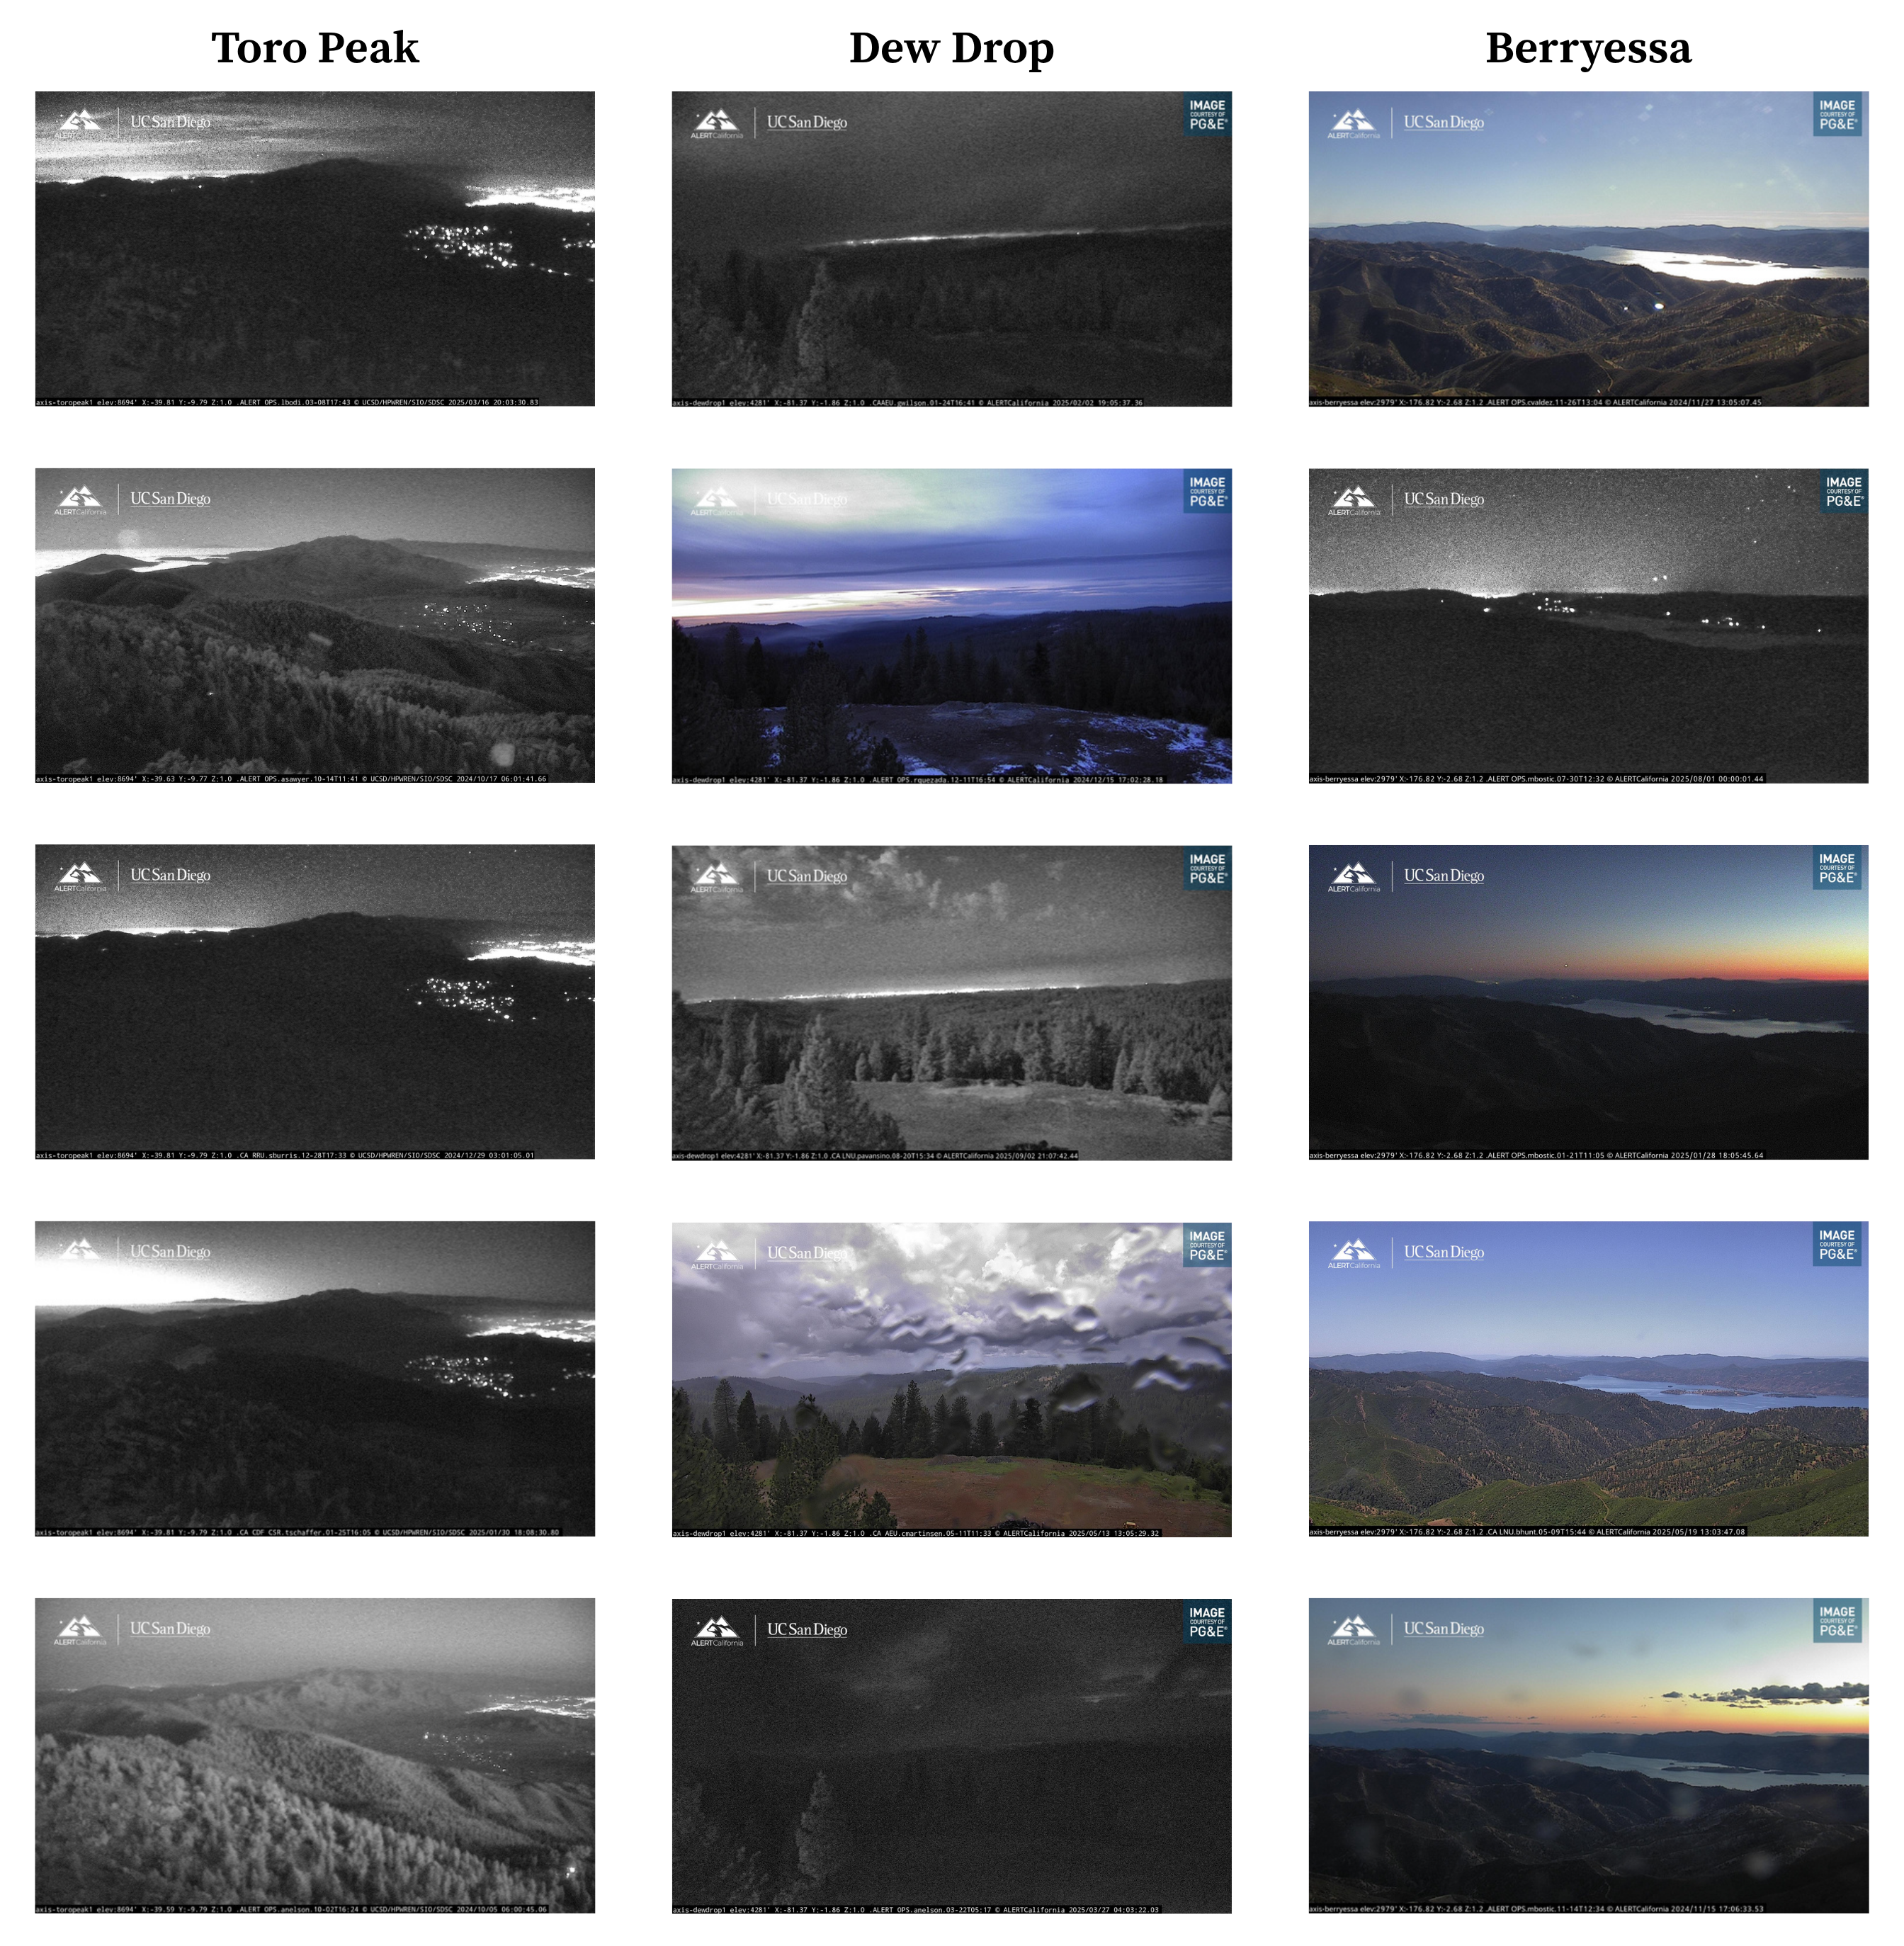
\includegraphics[width=1\linewidth]{figures/false_positives.png}
    \caption{A subset of false positive frames from each of the unseen camera locations.}
    \label{fig:false_positives}
\end{figure}

\subsection{Limitations and Future Work}

While the final multi-camera model demonstrates strong performance across the three cameras in the training set and moderate generalization to unseen landscapes, its scope is limited by the small number of cameras used in this study. With only three cameras in the final training set, the model cannot yet support the full scale of ALERTCalifornia's growing network of over 1,200 cameras. Our limited dataset does not encompass the full range of diverse landscapes and environmental conditions present across the entire camera network, leaving it vulnerable to misclassification errors in novel contexts. Future work should expand the training set to include a larger, more representative set of cameras spanning diverse landscapes and climates. This would ensure stronger generalization across a broader range of environmental conditions.


Another limitation is the aggregation of our 4-level image severity labels into a binary Normal and Abnormal classification. While this choice simplified our model training and evaluation, it also discards information that could be valuable when observing borderline cases or prioritizing maintenance. In practical deployment scenarios, a severity scale provides richer and more actionable insights for operators to distinguish between minor degradation issues and critical failures. 

Another significant limitation is the construction of the labeled dataset. Despite our best efforts to maintain consistency through a defined annotation rubric and the use of a majority vote, the assessment of an anomalous event is inherently subjective. Given the diversity of the four annotators and the fact that the labeling work spanned multiple weeks, slight shifts in interpretation were unavoidable and unfortunately present in our final labeled dataset. 

To quantify this uncertainty, we measure inter-rater agreement using Krippendorff's $\alpha$, obtaining a value of 0.6939. We additionally examine the consistency of agreement across annotators by performing a leave-one-annotator-out sensitivity analysis, producing $\alpha$ values ranging from 0.6602 to 0.7645. These results indicate moderate variability in agreement across annotators, suggesting that annotator disagreement is not only driven by labeling mistakes, but also by subjective interpretations of severity. 

This ambiguity is most apparent in borderline cases, particularly for images exhibiting gradual degradation or visibility. As revealed by the false positives analysis, many nighttime frames proved difficult to categorize, especially during low visibility settings. We acknowledge this limitation likely introduced noise and uncertainty that may have affected both the model training and evaluation. Future work should invest more time and resources to uphold the integrity of the dataset, such as refining labeling guidelines or using confidence-based annotations. 

This study primarily investigates the discriminative ability of a classification model to distinguish between Normal and Abnormal frames. While we extract feature embeddings using a \ac{ViT}-Base encoder, the semantic structure of the resulting lower-dimensional feature space is not explicitly analyzed. An interesting extension of this work would be to examine how environmental factors such as illumination, time of day, season, and weather conditions are encoded within the embedding space. Such analyses could provide deeper insight into how the model represents complex visual and environmental patterns, enhancing interpretability and robustness. To further improve interpretability and operational value, future work could also explore multi-level classification or continuous severity scoring to capture varying levels of image quality issues. 

%%%%%%%%%%%%%%%%%%%%%%%%%%%%%%%%%%%%%%%%%%
\section{Conclusions}

We present a \ac{ViT}-based framework for detecting \ac{QoS} anomalies in ALERTCalifornia wildfire monitoring cameras. By pairing a \ac{ViT}-Base encoder with a lightweight classifier and a custom labeling scheme, we demonstrate the effectiveness of a supervised embedding-based approach for automated camera quality monitoring. The final multi-camera model generalizes moderately well to unseen camera locations, with an average balanced accuracy of $82.88\%$ and an average \ac{AUPRC} of 0.8054. These results are hopeful in the context of environmental monitoring, as the \ac{AUPRC} indicates strong discriminative ability across thresholds.

Our findings suggest that a supervised \ac{ViT}-Base framework provides a promising foundation for automated image quality assessment, but additional work is necessary to support scalability across a network as large as ALERTCalifornia's. In particular, current generalization and scalability evaluations are limited, and further testing is required to assess model performance across a broader range of environmental conditions and geographic landscapes. Future efforts should aim to evaluate performance across a larger subset of the camera network and investigate methods for reducing false positives while maintaining the high recall observed in this work. 

In a practical deployment setting, the proposed framework could be integrated into existing camera processing pipelines to continuously evaluate incoming frames and assign anomaly labels. Flagged alerts could then be sent to system operators for further inspection or maintenance, or used to adjust thresholds in downstream hazard detection systems. Ultimately, by supporting the automated detection of degraded camera feeds, this approach has the potential to improve the reliability and efficiency of large-scale monitoring operations.

%%%%%%%%%%%%%%%%%%%%%%%%%%%%%%%%%%%%%%%%%%
\vspace{6pt} 

%%%%%%%%%%%%%%%%%%%%%%%%%%%%%%%%%%%%%%%%%%
%% optional
%\supplementary{The following supporting information can be downloaded at \linksupplementary{s1}, Figure S1: title; Table S1: title; Video S1: title.}

% Only for journal Methods and Protocols:
% If you wish to submit a video article, please do so with any other supplementary material.
% \supplementary{The following supporting information can be downloaded at \linksupplementary{s1}, Figure S1: title; Table S1: title; Video S1: title. A supporting video article is available at doi: link.}

% Only used for preprtints:
% \supplementary{The following supporting information can be downloaded at the website of this paper posted on \href{https://www.preprints.org/}{Preprints.org}.}

% Only for journal Hardware:
% If you wish to submit a video article, please do so with any other supplementary material.
% \supplementary{The following supporting information can be downloaded at \linksupplementary{s1}, Figure S1: title; Table S1: title; Video S1: title.\vspace{6pt}\\
%\begin{tabularx}{\textwidth}{lll}
%\toprule
%\textbf{Name} & \textbf{Type} & \textbf{Description} \\
%\midrule
%S1 & Python script (.py) & Script of python source code used in XX \\
%S2 & Text (.txt) & Script of modelling code used to make Figure X \\
%S3 & Text (.txt) & Raw data from experiment X \\
%S4 & Video (.mp4) & Video demonstrating the hardware in use \\
%... & ... & ... \\
%\bottomrule
%\end{tabularx}
%}

%%%%%%%%%%%%%%%%%%%%%%%%%%%%%%%%%%%%%%%%%%
\authorcontributions{For research articles with several authors, a short paragraph specifying their individual contributions must be provided. The following statements should be used ``Conceptualization, X.X. and Y.Y.; methodology, X.X.; software, X.X.; validation, X.X., Y.Y. and Z.Z.; formal analysis, X.X.; investigation, X.X.; resources, X.X.; data curation, X.X.; writing---original draft preparation, X.X.; writing---review and editing, X.X.; visualization, X.X.; supervision, X.X.; project administration, X.X.; funding acquisition, Y.Y. All authors have read and agreed to the published version of the manuscript.'', please turn to the  \href{http://img.mdpi.org/data/contributor-role-instruction.pdf}{CRediT taxonomy} for the term explanation. Authorship must be limited to those who have contributed substantially to the work~reported.}

\funding{This work was supported in part by the California Department of Forestry and Fire Protection (CALFIRE) under award \#7CA04784, the Kinsella Innovation Fund, as well as the National Science Foundation under award \#CNS-1338192, MRI: Development of Advanced Visualization Instrumentation for the Collaborative Exploration of Big Data. Opinions, findings, and conclusions from this study are those of the authors, and do not necessarily reflect the opinions of the research sponsors.
}

% \institutionalreview{In this section, please add the Institutional Review Board Statement and approval number for studies involving humans or animals. You might choose to exclude this statement if the study did not require ethical approval. Please note that the Editorial Office might ask you for further information. Please add ``The study was conducted in accordance with the Declaration of Helsinki, and approved by the Institutional Review Board (or Ethics Committee) of NAME OF INSTITUTE (protocol code XXX and date of approval).” for studies involving humans OR ``The animal study protocol was approved by the Institutional Review Board (or Ethics Committee) of NAME OF INSTITUTE (protocol code XXX and date of approval).” for studies involving animals OR ``Ethical review and approval were waived for this study due to REASON (please provide a detailed justification).” OR ``Not applicable.” for studies not involving humans or animals.}

% \informedconsent{Any research article describing a study involving humans should contain this statement. Please add ``Informed consent was obtained from all subjects involved in the study.'' OR ``Patient consent was waived due to REASON (please provide a detailed justification).'' OR ``Not applicable'' for studies not involving humans. You might also choose to exclude this statement if the study did not involve humans.

% Written informed consent for publication must be obtained from participating patients who can be identified (including by the patients themselves). Please state ``Written informed consent has been obtained from the patient(s) to publish this paper.” if applicable.}

\dataavailability{Data is available at https://dsc180.dronelab.ucsd.edu} 

%\durcstatement{Current research is limited to the [please insert a specific academic field, e.g., XXX], which is beneficial [share benefits and/or primary use] and does not pose a threat to public health or national security. Authors acknowledge the dual-use potential of the research involving xxx and confirm that all necessary precautions have been taken to prevent potential misuse. As an ethical responsibility, authors strictly adhere to relevant national and international laws about DURC. Authors advocate for responsible deployment, ethical considerations, regulatory compliance, and transparent reporting to mitigate misuse risks and foster beneficial outcomes.}

% Only for journal Nursing Reports
%\publicinvolvement{Please describe how the public (patients, consumers, carers) were involved in the research. Consider reporting against the GRIPP2 (Guidance for Reporting Involvement of Patients and the Public) checklist. If the public were not involved in any aspect of the research add: ``No public involvement in any aspect of this research''.}
%
%% Only for journal Nursing Reports
%\guidelinesstandards{Please add a statement indicating which reporting guideline was used when drafting the report. For example, ``This manuscript was drafted against the XXX (the full name of reporting guidelines and citation) for XXX (type of research) research''. A complete list of reporting guidelines can be accessed via the equator network: \url{https://www.equator-network.org/}.}
%
%% Only for journal Nursing Reports
%\useofartificialintelligence{Please describe in detail any and all uses of artificial intelligence (AI) or AI-assisted tools used in the preparation of the manuscript. This may include, but is not limited to, language translation, language editing and grammar, or generating text. Alternatively, please state that “AI or AI-assisted tools were not used in drafting any aspect of this manuscript”.}

% \acknowledgments{In this section, you can acknowledge any support given that is not covered by the author contribution or funding sections. This may include administrative and technical support, or donations in kind (e.g., materials used for experiments). Where GenAI has been used for purposes such as generating text, data, or graphics, or for study design, data collection, analysis, or interpretation of data, please add ``During the preparation of this manuscript/study, the author(s) used [tool name, version information] for the purposes of [description of use]. The authors have reviewed and edited the output and take full responsibility for the content of this publication.”}

\conflictsofinterest{The authors declare no conflicts of interest.} 

%%%%%%%%%%%%%%%%%%%%%%%%%%%%%%%%%%%%%%%%%%
%% Optional

%% Only for journal Encyclopedia
%\entrylink{The Link to this entry published on the encyclopedia platform.}

\abbreviations{Abbreviations}{%
The following abbreviations are used in this manuscript:\\

\noindent 
\begin{acronym}
  \acro{QoS}{quality of service}
  \acro{CNNs}{convolutional neural networks}
  \acro{GANs}{generative adversarial networks}
  \acro{AUPRC}{area under the precision-recall curve}
  \acro{ViT}{vision transformer}
  \acro{PCA}{principal component analysis}
  \acro{PC}{principal component}
  \acro{MLP}{multi-layer perceptron}
  \acro{GPU}{graphics processing unit}
  \acro{ORR}{operationally relevant region}
  \acro{SD}{standard deviation}
  \acro{PRC}{precision-recall curve}
  \acro{DeepSAD}{deep semi-supervised anomaly detection}
  \acro{H-SAD}{hierarchical semi-supervised anomaly detection}
\end{acronym}
}

%%%%%%%%%%%%%%%%%%%%%%%%%%%%%%%%%%%%%%%%%%
%% Optional
\appendixstart
\appendix
\section{Triplet Margin Loss}
\label{app:marginloss}
The triplet margin loss is a function that aims to bring points of similar classes closer together, while pushing dissimilar points further away \cite{Schroff_2015_CVPR}. First, a dataset of triplets of the form ($A, P, N$) is computed, where A is an anchor point, P is a positive point (of the same class as A), and N is a negative point (of a different class from A). Generally, the loss is computed on a function $f(x)$ which maps a point $x$ to a finite-dimensional Euclidean space in order to optimize it. In our case, each “point” is an input image, each of which is represented as a tensor of size 224 x 224 x 3. The anchor point A can belong to either the Normal or Abnormal class in our case. If A is Normal, then the positive point P will also be some Normal point, while N will be some Abnormal point. Conversely, if A is Abnormal, then P will also be Abnormal, while N will be Normal. The function $f(x)$ on which we compute the loss is our baseline encoder model, which maps these images into vectors f(A), f(P), and f(N), each of which exists in $\mathbb{R}^{768}$. We refer to these vectors as the embeddings of A, P, and N, respectively. Formally, we express this setup as follows:

\[
\mathcal{D} = \{(A_i, P_i, N_i)\}_{i=1}^m,\qquad
y_{A_i} = y_{P_i}),\qquad y_{A_i} \neq y_{N_i},
\]

\[
A_i, P_i, N_i \in \mathbb{R}^{224 \times 224 \times 3}, \qquad
f : \mathbb{R}^{224 \times 224 \times 3} \to \mathbb{R}^{768},
\]

\[
f(A_i),\, f(P_i),\, f(N_i) \in \mathbb{R}^{768}.
\]

where $\mathcal{D}$ is the dataset of triplets and $y_x$ is the label for some point x. The goal of training is to ensure that for any triplet $(A_i, P_i, N_i)$ selected from $\mathcal{D}$, the distance from $f(A_i)$ to $f(P_i)$ is less than the distance from $f(A_i)$ to $f(N_i)$ by some margin $\alpha$. More formally, for any triplet ($A_i, P_i, N_i$), the following constraint is satisfied: 

$$
\|f(A_i) - f(P_i)\|_2^2 + \alpha < \|f(A_i) - f(N_i)\|_2^2
$$

where $\alpha$ is the hyperparameter for the margin. The loss function we must minimize is the following: 

$$
L = \sum_{i=1}^{m} \max \left( \|f(A_i) - f(P_i)\|_2^2 - \|f(A_i) - f(N_i)\|_2^2 + \alpha, 0 \right)
$$

\section{Triplet Mining}
\label{app:mining}

Triplet mining is leveraged to optimize the triplets used while computing triplet margin loss. The set of all possible triplets of the form ($A, P, N$) is very large, and computing a loss function based on all of them would be very computationally intensive. In their paper on FaceNet, Schroff et al. only include a given triplet ($A_i, P_i, N_i$) in the loss computation when $N^i$ is a hard negative: that is, a negative point whose embedding $f(N^i)$ lies inside the margin \cite{Schroff_2015_CVPR}. This leads to faster convergence than a training process that uses easy negatives: negative points whose embeddings already lie outside the margin. However, the authors of FaceNet also find that training on the hardest negatives early on can lead the algorithm to converge to a bad local minimum early in training, resulting in model collapse. Therefore, they choose to train on triplets with semi-hard negatives: those whose embeddings lie inside the margin, but are still further from that of the positive point \cite{Schroff_2015_CVPR}. Figure~\ref{fig:tml} demonstrates the relationships between these types of points in the embedding space. More formally, a triplet ($A_i, P_i, N_i$) is semi-hard if it satisfies the following constraint: 

$$
\|f(A^{(i)}) - f(P^{(i)})\|_2^2 < \|f(A^{(i)}) - f(N^{(i)})\|_2^2 < \|f(A^{(i)}) - f(P^{(i)})\|_2^2 + \alpha
$$

In our implementation, we train on \textit{all} triplets (those with Normal anchors and those with Abnormal anchors) with semi-hard negatives in order to maximize the information gained during training, while also ensuring that our encoder does not degenerate. 

\begin{figure}[H]
    \centering
    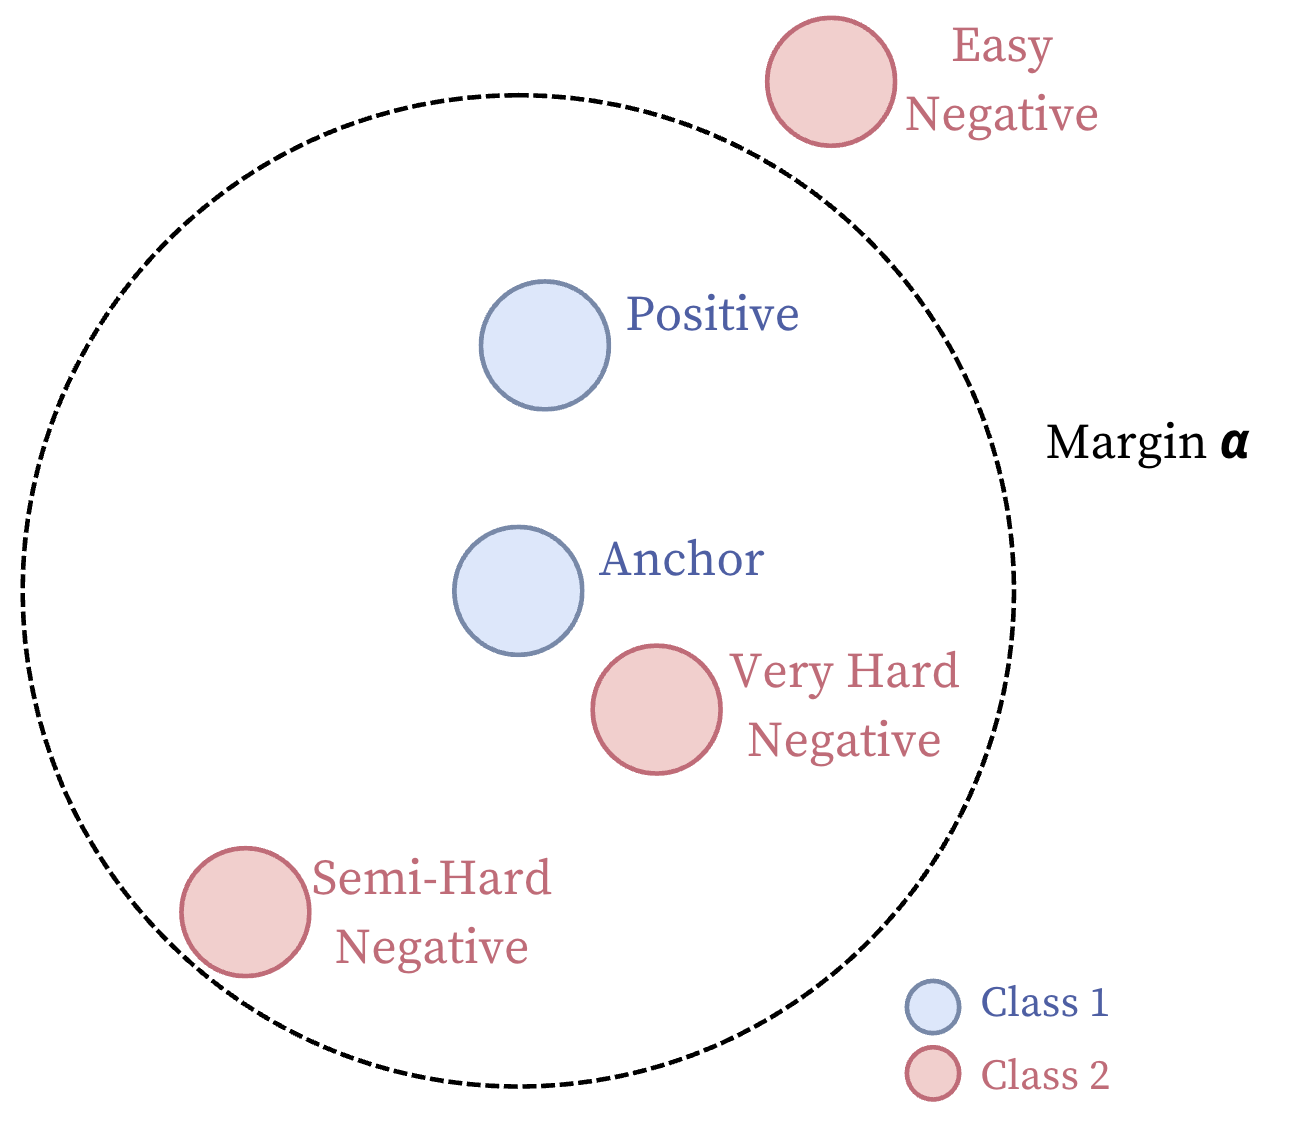
\includegraphics[width=0.6\linewidth]{figures/tml.png}
    \caption{A diagram showing how the embeddings of different types of negative points exist in feature space during computation of triplet margin loss. Easy negatives' embeddings lie outside the margin $\alpha$; they already satisfy the triplet constraint. In contrast, hard negatives' embeddings lie inside the margin. There are two subtypes: semi-hard negatives, whose embeddings lie further away from the anchor than the positive point, and very hard negatives, whose embeddings lie closer to the anchor than the positive point.}
    \label{fig:tml}
\end{figure}

\section{\ac{DeepSAD} Loss}
\label{app:deepsad}
The Deep Semi-supervised Anomaly Detection (\ac{DeepSAD}) loss function is an objective developed by Ruff et. al~\cite{ruff2019deep}. It accepts a training dataset of both labeled and unlabeled samples as input, with the labeled samples having a binary classification of Normal or Abnormal. It aims to pull Normal points close to some cluster center in hyperspace, while pushing Abnormal points outwards.

Suppose we have a neural network $\phi(\cdot;\mathcal{W}): \mathcal{X} \rightarrow \mathcal{Z}$ which maps data from an input space $\mathcal{X} \subseteq \mathbb{R}^D$ to an output space $\mathcal{Z} \subseteq \mathbb{R}^d$. This network contains $K$ hidden layers, with a corresponding set of weights $\mathcal{W} = \{W^1, W^2, ..., W^K\}$. Additionally, suppose we have some dataset $X = \{x_1, x_2, ..., x_{n+m}\}$, which contains both labeled and unlabeled data. We define the subset $L \subset X = \left\{(\tilde{x}_j, y_j) | \tilde{x}_j \in X, y_j \in \{1, -1\}\right\}_{j=1}^{m}$, which contains only labeled data. Here, $y_j = 1$ means the corresponding image $\tilde{x_j}$ is Normal, while $y_j = -1$ means the corresponding image $\tilde{x_j}$ is Abnormal. We also define the subset $U \subset X = \{x_i\}_{i=1}^{n}$ which contains only unlabeled data. The \ac{DeepSAD} objective function is defined as follows:

\[\mathcal{L}_{SAD} := \frac{1}{n + m}\sum_{x_i \in U}{\|\phi(x_i;\mathcal{W}) - c\|^2} + \frac{\eta}{n + m}\sum_{(\tilde{x_j}, y_j) \in L}{(\|\phi(\tilde{x_j};\mathcal{W}) - c\|^{2})^{y_j}} + \lambda\sum_{\ell = 1}^{K}{\|W^{\ell}\|^2_F}\]

where $c \in \mathbb{R}^d$ denotes the hypersphere cluster center around which the points are mapped~\cite{ruff2019deep}.

Crucially, this function assumes that most of the points in $X$ are Normal in ground truth. This allows us to incorporate the first term, which penalizes the distance from the unlabeled samples to the cluster center. This means that the network is incentivized to learn a set of weights $\mathcal{W}$ that pulls most unlabeled points close to the cluster center. 

The second term utilizes the information from the labeled data to push known Abnormal points away. The data labeled as Normal are pulled even closer to the center, while those labeled Abnormal are pushed further away. The hyperparameter $\eta$ controls the influence of the second term relative to the first. Setting $\eta$ > 1 leads to the emphasis of labeled data over unlabeled data, while setting $\eta$ < 1 emphasizes unlabeled data over labeled data. The inclusion of this term is predicated on a second assumption--that Abnormal images vary greatly in appearance, while Normal images tend to be more similar to each other~\cite{ruff2019deep}. 

The final term is a weight regularization term, whose influence is controlled by the hyperparameter $\lambda$.

\section{\ac{H-SAD} Loss}
\label{app:hsad}

The Hierarchical Semi-Supervised Anomaly Detection (\ac{H-SAD}) loss function is an objective that we have developed. It extends the \ac{DeepSAD}~\cite{ruff2019deep} loss function to a 4-point ordinal labeling scale. That is, it aims to pull Clear points close to some cluster center in hyperspace, while pushing non-Clear points outwards to varying degrees, depending on the severity of the anomaly. 

For computation, we convert our labels to numeric values as follows:
\begin{itemize}
\item Points with a label of Clear receive a numeric label of 1,
\item Points with a label of Minor receive a numeric label of 2,
\item Points with a label of Major receive a numeric label of 3, and
\item Points with a label of Severe receive a numeric label of 4.
\end{itemize}

Suppose we have a neural network $\phi(\cdot;\mathcal{W}): \mathcal{X} \rightarrow \mathcal{Z}$ which maps data from an input space $\mathcal{X} \subseteq \mathbb{R}^D$ to an output space $\mathcal{Z} \subseteq \mathbb{R}^d$. This network contains $K$ hidden layers, with a corresponding set of weights $\mathcal{W} = \{W^1, W^2, ..., W^K\}$. Additionally, suppose we have some dataset $X = \{x_1, x_2, ..., x_{n+m}\}$, which contains both labeled and unlabeled data. We define the subset $L \subset X = \left\{(\tilde{x}_j, y_j) | \tilde{x}_j \in X, y_j \in \{1, 2,3, 4\}\right\}_{j=1}^{m}$, which contains only labeled data. We also define the subset $U \subset X = \{x_i\}_{i=1}^{n}$ which contains only unlabeled data. We create a binary classifier on the ground-truth labels:
\[b(y_i) = \begin{cases}
    1 & \text{if } y \in \{1,2\} \\
    -1 & \text{if } y \notin \{1,2\}
\end{cases}\]

which aggregates the labeled data into Normal (1) and Abnormal (-1) classes. We then define the following objective functions:
\[\mathcal{L}_{clear} := \frac{1}{n}\sum_{x_i \in U}{\|\phi(x_i;\mathcal{W}) - c_C\|^2} + \frac{\eta}{m}\sum_{(\tilde{x_j}, y_j) \in L}{(\|\phi(\tilde{x_j};\mathcal{W}) - c_C\|^{2})^{b(y_j)}}\]
and
\[\mathcal{L}_{anom} := \frac{1}{|A|}\sum_{j \in A}{\|\phi(\tilde{x_j};\mathcal{W}) - c_{y_j}\|^2}\]
such that:
\[\mathcal{L}_{HSAD} = \mathcal{L}_{clear} + \alpha\mathcal{L}_{anom} + \lambda\sum_{\ell = 1}^{K}{\|W^{\ell}\|^2_F}\]
where:
\begin{itemize}
\item $A = \left\{j | y_j \in \{2,3,4\}\right\}$ denotes the set of all indices for non-Clear labeled data,
\item $c_C \in \mathbb{R}^d$ denotes the hypersphere cluster center for Clear points,
\item $c_k \in \mathbb{R}^d$ denotes the hypersphere cluster center of class $k$ for $k \in \{2,3,4\}$
\end{itemize}

$\mathcal{L}_{clear}$ is adapted from the \ac{DeepSAD} objective function with some modifications. First, the unlabeled points are pulled towards the cluster center for Clear data, which have a label of 1; in the \ac{DeepSAD} equivalent, they would be pulled towards a cluster center for Normal points, which have a label of 1 or 2. Secondly, we binarize the labels before using them in the second term. Since the labels used for training with the \ac{DeepSAD} objective are already binary, this step is not needed in that case. 

$\mathcal{L}_{clear}$, like the \ac{DeepSAD} objective, relies on the assumption that the Normal data in $X$ vastly outnumber the Abnormal data. With this assumption, any unlabeled points are assumed to be Normal. Thus, the first term attempts to pull all unlabeled points towards the cluster center of Normal points.  

The second term of $\mathcal{L}_{clear}$ utilizes the information from the labeled data to push Abnormal points away. The data labeled as Normal are pulled closer to the center, while those labeled Abnormal are pushed further away. The hyperparameter $\eta$ controls the influence of the second term relative to the first.

In the 4-point ordinal case, the classes that comprise the Abnormal class--namely Major Anomalies and Severe Anomalies--contain several images that look similar to one another. This contradicts the second assumption of the \ac{DeepSAD} objective: that Abnormal images vary greatly in appearance. To circumvent this, we incorporate a second sub-function $\mathcal{L}_{anom}$, which seeks to bring non-Clear data closer to other data in the same class. This allows the embedding space to achieve minimal intra-class separation, as the other terms seek to maximize the separation between Normal and Abnormal data. The hyperparameter $\alpha$ controls the influence of $\mathcal{L}_{anom}$ relative to $\mathcal{L}_{clear}$. 

The final term is a weight regularization term, whose influence is controlled by the hyperparameter $\lambda$.

%%%%%%%%%%%%%%%%%%%%%%%%%%%%%%%%%%%%%%%%%%
%\isPreprints{}{% This command is only used for ``preprints''.
\begin{adjustwidth}{-\extralength}{0cm}
%} % If the paper is ``preprints'', please uncomment this parenthesis.
%\printendnotes[custom] % Un-comment to print a list of endnotes

\reftitle{References}

% References must be numbered in order of appearance in the text (including citations in tables and legends) and listed individually at the end of the manuscript. We recommend preparing the references with a bibliography software package, such as EndNote, ReferenceManager or Zotero, to avoid typing mistakes and duplicated references. Include the digital object identifier (DOI) for all references where available.
% Please provide either the correct journal abbreviation (e.g. according to the “The list of Title Word Abbreviations” https://portal.issn.org/ltwa) or the full name of the journal. 
% Citations and references in the Supplementary Materials are permitted provided that they also appear in the reference list here. 
% In the text, reference numbers should be placed in square brackets [ ] and placed before the punctuation; for example, [1], [1–3] or [1,3]. For embedded citations in the text with pagination, use both parentheses and brackets to indicate the reference number and page numbers; for example, [5] (p. 10), or [6] (pp. 101–105).

%=====================================
% References, variant A: external bibliography
%=====================================
\bibliography{reference}

% If authors have biography, please use the format below
%\section*{Short Biography of Authors}
%\bio
%{\raisebox{-0.35cm}{\includegraphics[width=3.5cm,height=5.3cm,clip,keepaspectratio]{Definitions/author1.pdf}}}
%{\textbf{Firstname Lastname} Biography of first author}
%
%\bio
%{\raisebox{-0.35cm}{\includegraphics[width=3.5cm,height=5.3cm,clip,keepaspectratio]{Definitions/author2.jpg}}}
%{\textbf{Firstname Lastname} Biography of second author}

% For the MDPI journals use author-date citation, please follow the formatting guidelines on http://www.mdpi.com/authors/references
% To cite two works by the same author: \citeauthor{ref-journal-1a} (\citeyear{ref-journal-1a}, \citeyear{ref-journal-1b}). This produces: Whittaker (1967, 1975)
% To cite two works by the same author with specific pages: \citeauthor{ref-journal-3a} (\citeyear{ref-journal-3a}, p. 328; \citeyear{ref-journal-3b}, p.475). This produces: Wong (1999, p. 328; 2000, p. 475)

%%%%%%%%%%%%%%%%%%%%%%%%%%%%%%%%%%%%%%%%%%
%% for journal Sci
%\reviewreports{\\
%Reviewer 1 comments and authors’ response\\
%Reviewer 2 comments and authors’ response\\
%Reviewer 3 comments and authors’ response
%}
%%%%%%%%%%%%%%%%%%%%%%%%%%%%%%%%%%%%%%%%%%
\PublishersNote{}
%\isPreprints{}{% This command is only used for ``preprints''.
\end{adjustwidth}
%} % If the paper is ``preprints'', please uncomment this parenthesis.
\end{document}

